% $Id$
\documentclass[10pt]{article}
\def\typeofdocument{article}    % ``article'' or ``report''
\usepackage{epsfig}
\usepackage{dcolumn}
\usepackage{alltt}
\usepackage{rotating}

% Delete in final version of paper.
\newcommand{\comment}[1]{\textbf{[[#1]]}}
% Delete above in final version of paper


\newcommand{\pcp}{\mbox{\textsf{PCp}$^3$}}

\def\numpackages{26}
\def\numlines{1.4 million}      % 1372618 as of 5 Feb 1999
% \def\numlinesexact{1.4 million}
\def\numlinesalmost{1.4 million}
% \def\numlinesncnbexact{1 million} % 973877 as of 5 Feb 1999

\def\nummacrodefs{26182}        % as of 5 Feb 1999
\def\nummacronames{21968}

\def\numdependpackages{25}
\def\numdependmacronames{19945}

\newcommand{\pkg}[1]{\textsf{#1}}
\newcommand{\file}[1]{\texttt{#1}}
\newcommand{\ppd}[1]{\texttt{\##1}}

% the "fullpage" package does almost the same thing
% as the below lines-- it doesn't make things quite as
% tall or wide, but is generally what I use
% \usepackage{fullpage}
\marginparwidth 0pt
\oddsidemargin  0pt
\evensidemargin 0pt
\marginparsep 0pt
\topmargin   0pt
\headsep 0pt
\headheight 0pt
\textwidth   6.5 in
\textheight  9 in

%% Figures
\newcommand{\captionsmall}[1]{\caption[]{\small #1}}
% Changing this to .9 shoves lots of figures to the end of the document; why?
\renewcommand{\floatpagefraction}{.8} %default .5
% \renewcommand{\floatpagefraction}{.9} %default .5
% Avoid putting all figures at end of text.
\renewcommand{\textfraction}{.1}  % .2 is the default
\renewcommand{\topfraction}{.9}   % .7 is the default
%% Get a line between figures at the top of the page and the text
 \makeatletter
 \def\topfigrule{\kern3\p@ \hrule \kern -3.4\p@} % the \hrule is .4pt high
 \def\botfigrule{\kern-3\p@ \hrule \kern 2.6\p@} % the \hrule is .4pt high
 \makeatother


%%% end of header
%%%%%%%%%%%%%%%%%%%%%%%%%%%%%%%%%%%%%%%%%%%%%%%%%%%%%%%%%%%%%%%%%%%%%%%%%%%

\begin{document}
% \bibliographystyle{plain}
\bibliographystyle{alpha}

\title{An Empirical Analysis of C Preprocessor Use}

\author{Michael D. Ernst \and Greg J. Badros \and David Notkin}

\date{Revision of Technical Report UW-CSE-97-04-06 (original date April 22, 1997) \\
Department of Computer Science and Engineering \\
University of Washington \\
Box 352350, Seattle, WA  98195-2350  USA \\
{\small \{{\tt mernst},{\tt gjb},{\tt notkin}\}{\tt @cs.washington.edu}} \\
31 March 1999}  

\maketitle

\begin{abstract}
  This is the first empirical study of the use of the C macro preprocessor,
  Cpp.  To determine how the preprocessor is used in practice, this paper
  analyzes {\numpackages} packages comprising {\numlinesalmost} lines of
  publicly available C code.  We determine the incidence of C preprocessor
  usage\,---\,whether in macro definitions, macro uses, or dependences upon
  macros\,---\,that is complex, potentially problematic, or inexpressible
  in terms of other C or C++ language features.  We taxonomize these
  various aspects of preprocessor use and particularly note data that are
  material to the development of tools for C or C++, including translating
  from C to C++ to reduce preprocessor usage.  Our results show that while
  most Cpp usage follows fairly simple patterns, an effective program
  analysis tool must address the preprocessor.
  
  The intimate connection between the C programming language and Cpp, and
  Cpp's unstructured transformations of token streams, often hinder
  programmer understanding of C programs and tools built to engineer C
  programs, such as compilers, debuggers, call graph extractors, and
  translators.  Most tools make no attempt to analyze macro usage, but
  simply preprocess their input, which results in a number of negative
  consequences; an analysis that takes Cpp into account is preferable, but
  building such tools requires an understanding of actual usage.
  Differences between the semantics of Cpp and those of C can lead to
  subtle bugs stemming from the use of the preprocessor, but there are no
  previous reports of the prevalence of such errors.  Use of C++ can reduce
  some preprocessor usage, but such usage has not been previously measured.
  Our data and analyses shed light on these issues and others related to
  practical understanding or manipulation of real C programs.  The results
  are of interest to language designers, tool writers, programmers, and
  software engineers.
\end{abstract}

%\noindent
%Keywords: C preprocessor, Cpp, C, C++, program understanding, file
%inclusion, macro, macro substitution, conditional compilation, empirical study


\bigskip

\section{Coping with the Preprocessor}

The C programming language~\cite{KernighanR88,Harbison91} is
incomplete without its macro preprocessor, Cpp.  Cpp can be used to
define constants, define new syntax, abbreviate repetitive or
complicated constructs, support conditional compilation, and 
reduce or eliminate reliance on a compiler implementation to perform 
many optimizations.
%propagate symbolic
%constants, open-code functions, eliminate dead code, and short-circuit
%constant tests.
Cpp also permits system dependences to be made explicit, resulting in
a clearer separation of those concerns.  In addition, Cpp permits a single
source to contain multiple different dialects of C, such as both
K\&R-style and ANSI-style declarations.

%The C programming language~\cite{KernighanR88,Harbison91} is incomplete
%without its macro preprocessor, Cpp.  By supplying such facilities as file
%inclusion, definition of constants and macros, and conditional compilation,
%Cpp can define new syntax, abbreviate repetitive or complicated constructs,
%or eliminate reliance on a compiler implementation to propagate symbolic
%constants, open-code functions, eliminate dead code, and short-circuit
%constant tests.  Cpp also permits system dependences to be made explicit
%and tested, resulting in a clearer separation of concerns.  In addition,
%Cpp permits a single source to contain multiple different dialects of C,
%such as supporting both K\&R-style and ANSI-style declarations.

% Indeed, one cannot write practical C programs without these facilities.

While disciplined use of the preprocessor can reduce programmer effort
and improve portability, performance, or readability, Cpp is widely
viewed as a source of difficulty for understanding and modifying C
programs.  Cpp's lack of structure\,---\,its inputs and outputs are
token streams\,---\,engenders flexibility but allows arbitrary source
code manipulations that may complicate understanding of the program by
programmers and tools.  In the worst case, the preprocessor makes
merely determining the program text as difficult as determining the
output of an ordinary program.  The designer of the C++ language,
which shares C's preprocessor, also noted these problems:
``Occasionally, even the most extreme uses of Cpp are useful, but its
facilities are so unstructured and intrusive that they are a constant
problem to programmers, maintainers, people porting code, and tool
builders''~\cite[p.~424]{Stroustrup-DesignEvolution}.

Given the wide range of possible uses of the preprocessor, our
research addresses the question of how it is actually used in
practice.  Our statistical analysis of {\numpackages} C programs
comprising {\numlinesalmost} lines of code provides significant
insights with respect to this question.  We are not aware of any
similar data or analysis in the literature.

We had three initial motivations for pursuing this line of research.
First, we wanted to evaluate the potential for reducing
preprocessor usage when converting a program from C to C++.
Second, we wanted to know how difficult it would be to produce a
framework for preprocessor-aware tools.  Third, we wanted to develop a
tool for identifying common pitfalls in the use of macros.

These motivations drove our selection of the data we extracted and the
analyses that we performed.  Our data, our analyses, and our insights
take substantive steps towards addressing these three issues.
Overall, our analysis confirms that the C preprocessor is used in
exceptionally broad and diverse ways, complicating the development of
C programming support tools.  About two-thirds of macro definitions
and uses are relatively simple, of the variety that a programmer could
understand through simple but tedious effort or that a relatively
unsophisticated tool could manage (although in practice very few even
try).  Though these simple kinds of macros predominate, the preprocessor is so
heavily used that it is worthwhile to understand, annotate, or
eliminate the remaining one-third of the macros; these are the macros which are most likely
to cause difficulties.

%We had two initial motivations for pursuing this line of research.
%One, we wanted to know how difficult it would be, in practice, to
%vastly reduce the usage of the preprocessor when converting a program
%from C to C++.  Two, we wanted to know how difficult it would be to
%produce a tool framework that would simplify the development of tools
%that are knowledgeable about the preprocessor.
%
%Our data and our insights take substantive steps towards answering
%these two questions; throughout the body of the paper, we use these
%two issues as the primary basis for putting the data into context.  We
%believe, however, that the utility of the data could extend further.
%
%Overall, our analysis confirms that the C preprocessor is used in
%exceptionally broad and diverse ways, complicating the development of
%C programming support tools.  About two-thirds of macro definitions
%and uses are relatively simple, of the variety that a programmer could
%understand through simple but tedious effort or that a relatively
%unsophisticated tool could manage (although in practice very few even
%try).  While these kinds of macros predominate, the preprocessor is so
%heavily used that it is worthwhile to understand, annotate, or
%eliminate the remaining one-third of the macros, which are most likely
%to cause difficulties.

Section~\ref{sec:background} provides additional detail about the
difficulties imposed by the preprocessor.
Section~\ref{sec:methodology} describes our experimental methodology.
Sections~\ref{sec:first-content-section}--\ref{sec:last-content-section}
present the bulk of results about macro preprocessor use.
Section~\ref{sec:related} discusses related work, and
Section~\ref{sec:easier-to-understand} suggests techniques for mitigating
the negative impact of Cpp on program understanding.
Section~\ref{sec:future-work} presents avenues for future work, and the
concluding section discusses the relevance of the research.


\section{Background}\label{sec:background}

Tools\,---\,and, to a lesser degree, software engineers\,---\,have
three options for coping with Cpp.  They may ignore preprocessor
directives altogether, accept only post-processed code (usually by
running Cpp on their input), or attempt to emulate the preprocessor by
tracking macro definitions and the value of conditional compilation tests.
Each approach has different strengths and weaknesses.

\begin{itemize}

\item Ignoring preprocessor directives is an option for tools that produce
  approximate information, such as those based on lexical or approximate
  parsing techniques.  However, if accurate information about function
  extents, scope nesting, declared variables and functions, and other
  aspects of a program is required, the preprocessor cannot be ignored.

\item Operating on post-processed code, the most common strategy, is
  simple to implement, but the tool's input differs from what the
  programmer sees.  Even when line number mappings are maintained,
  other information is lost in the mapping back to the original source
  code.  Source-level debuggers have no symbolic names or types for
  constants and functions introduced via {\tt \#define}, nor can tools
  trace or set breakpoints in function macros, as they can for
  ordinary functions (even those that have been
  inlined~\cite{Zellweger83:TR}).  An example of a tool working on the
  post-processed code is the use of type inferencing to produce C++
  function templates from C; however, the input ``has been
  preprocessed so that all include files are incorporated and all
  macros expanded''~\cite[p.~145]{Siff-fse96}.  Such preprocessing may
  limit the readability and reusability of the resulting C++
  templates.  Another example is that call graph extractors generally
  work in terms of the post-processed code, even when a human is the
  intended consumer of the call graph~\cite{Murphy-icse18}.


  A tool that manipulates post-processed code cannot be run on a
  program that will not preprocess on the platform on which the tool
  is being run.  Some such tools also reject ill-formed programs
  that will not compile without errors.  These constraints complicate
  porting and maintenance, two of the situations in which program
  understanding and transformation tools are most likely to be needed.
  Additionally, a tool supplied with only one post-processed
  instantiation of the source code cannot reason about the program as
  a whole, only about the version that results from one particular set
  of preprocessor variables.  For instance, a bug in one configuration
  may not be discovered despite exhaustive testing or analysis of
  other configurations.



%  Some tools even leave the software engineer responsible for inferring the
%  mapping between the original and the post-processed source, which is an
%  undesirable and error-prone situation.
  

% that do not incorporate particular code
%  or do not admit particular execution paths.

\item The final option, emulating the preprocessor, is fraught with
  difficulty.  Macro definitions consist of complete tokens but need not be
  complete expressions or statements.  Conditional compilation and
  alternative macro definitions lead to very different results from a
  single original program text.  Preprocessing adds complexity to an
  implementation, which must trade off performing preprocessing against
  maintaining the code in close to its original form.  Extracting structure
  from macro-obfuscated source is not a task for the faint-hearted.
  Despite these problems, in many situations only some sort of
  preprocessing or Cpp analysis can produce useful answers.

\end{itemize}

%All three approaches would be unnecessary if programs did not use
%preprocessor directives.  This is exactly what Stroustrup suggests:
%\begin{quote}
%  I'd like to see Cpp abolished.  However, the only realistic and
%  responsible way of doing that is first to make it redundant, then
%  encourage people to use the better alternatives, and {\em then\/}\,---\,years
%  later\,---\,banish Cpp into the program development environment with the
%  other extra-linguistic tools where it
%  belongs~\cite[p.~426]{Stroustrup-DesignEvolution}.
%\end{quote}
%C++ contains features\,---\,such as constant variables, inline functions,
%templates, and reference parameters\,---\,that obviate many uses of Cpp.
%Thus, translation to C++ is a path for partial elimination of Cpp.
%This study indicates the
%feasibility\,---\,and our framework for analyzing preprocessor usage
%provides a basis for the development\,---\,of an automatic translator with
%two attractive properties.  It would take as input C programs complete with
%preprocessor directives, and it would map many uses of directives into C++
%language features.  (It is not 
%practical to eliminate all uses of Cpp.  For example, C++ currently
%provides no replacement for the {\tt \#include} directive, or for
%stringization or pasting.  Macros that cannot be eliminated might be
%annotated with their types or 
%effects on parser or program state, so that even tools that do no Cpp
%analysis can operate correctly on such programs.)

Choices among these options are currently made in the absence of
an understanding of how Cpp is used in practice.
While  Cpp's potential pitfalls are well-known, no
previous work has examined actual use of the C preprocessor to
determine whether it presents a practical or merely theoretical
obstacle to program understanding, analysis, and modification.  This
paper fills that gap by examining Cpp use in {\numpackages} programs
comprising {\numlines} lines of source code.

The analysis focuses on potential pitfalls that complicate the work of
software engineers and tool builders:
\begin{description}\itemsep 0pt \parskip 0pt
\item[high total use {\rm (Sections~\ref{sec:directives}, \ref{sec:macro-usage}, and~\ref{sec:dependence}):}]
  Heavy use of either macro substitution or conditional compilation can
  overwhelm a human or tool.  Lines that
  depend on many macros or macros that affect many lines are more
  likely to be problematic.
\item[complicated bodies {\rm (Section~\ref{sec:categorization}):}]
  A macro body need not expand to a complete C syntactic entity (such as a
  statement or expression).
\item[extra-linguistic features {\rm (Section~\ref{sec:extra-linguistic}):}]
  A macro body may exploit features of the preprocessor not available in C,
  such as stringization, token pasting, or use of free variables.
\item[macro pitfalls {\rm (Section~\ref{sec:lint}):}]
  Macros introduce new varieties of programming errors, such as
  function-like macros that fail to swallow a following semicolon and
  macros that modify, or fail to parenthesize, uses of their arguments.
\item[multiple definitions {\rm (Sections~\ref{sec:mult-def}--\ref{sec:inconsistent}):}]
  Uncertainty about the expansion of a macro makes it harder to confidently
  understand the
  actual program text.  Even more problematically, two definitions of a
  macro may be incompatible, for instance if one expands to a statement and the
  other to an expression or type.
\item[inconsistent usage {\rm (Section~\ref{sec:inconsistent-usage}):}]
  A macro used both for conditional compilation and to expand code is
  harder to understand than one used exclusively for one purpose.
\item[mixed tests {\rm (Section~\ref{sec:ccd}):}]
  A single Cpp conditional ({\tt \#if} directive) may test conceptually
  distinct conditions, making it difficult to perceive the
  test's purpose.
\item[variation in use{\rm :}]
  Preprocessor use varies widely.
  In the absence of a clear pattern of use or commonly-repeated paradigms,
  no obvious point of attack presents itself to eliminate most complexity
  with little effort.  We examine this issue throughout the \typeofdocument.
  %% No pattern according to package size, relative or absolute Cpp use, etc.
\end{description}

We report in detail on each of these aspects of preprocessor use,
indicating which are innocuous in practice and which problematic uses
appear more frequently.  We also taxonomize macro bodies, macro features,
macro errors, and conditional tests.  These taxonomies are more detailed,
and they more accurately reflect actual use, than previous work.

%%Numbers:
%% ``about one third'' comes from adding the extra-linguistic numbers (from
%% tbl-subset-properties.tex, 14.1%) and macro lint numbers (from
%% tbl-lint.tex, 22 or 23%); but I don't know the exact overlap of the two
%% numbers, so I am a big vague here.  2/5/99



% [[Point reader at conclusion/summary of results, at end of paper (and write
% that!).]]

% \subsection{Outline}
% 
% The remainder of this paper is organized as follows.
% 
% Section~\ref{sec:directives} reports the percentage of original C source
% code lines that are preprocessor directives, including a breakdown of the
% frequency of specific directives such as {\tt \#define}.  C programs
% commonly have preprocessor directives as over 10\% of their total lines,
% and over 20\% of the lines are directives in 3 of the {\numpackages}
% packages.
% 
% Section~\ref{sec:usage} reports how often each macro is defined and
% expanded.   Identifiers tend to be {\tt \#define}d relatively few times
% (96\% of macro identifiers have three or fewer definitions).  Many packages
% also have a significant number of macros that are never expanded, even
% disregarding system and library header files.
% 
% Section~\ref{sec:categorization} categorizes macro definitions according to
% their expansions; for example, macros may simply define a preprocessor
% symbol, define a literal, expand to a statement, etc.  We were particularly
% interested in determining the frequency of use of macros that are difficult
% to convert to other language features, such as those that string together
% characters as opposed to manipulating lexemes or syntactic units (less than
% .3\% of all macro definitions),
% those that expand to partial syntactic units such as unbalanced
% braces or partial declarations (.5\%), and others not 
% directly expressible in the programming language (about 4\%).
% 
% Section~\ref{sec:conclusion} discusses the relevance of the research,
% suggests techniques for mitigating the negative impact of Cpp on program
% understanding, and discusses avenues for future work, while
% Section~\ref{sec:related} discusses related work.



%Overall, our analysis confirms that the C preprocessor is used in
%exceptionally broad and diverse ways, complicating the development of C
%programming support tools.  On the other hand, the analysis also convinces
%us that, by extending our analysis framework with some class type
%inferencing techniques (similar to those used for C to C++
%translation~\cite{Siff-fse96} and for program
%understanding~\cite{OCallahan-icse97}), we can take significant
%steps towards a tool that usefully converts a high percentage of Cpp code
%into C++ language features.  We are interested not in translations
%that merely allow a C program to be compiled by a C++ compiler (which is
%usually easy, by intentional design of C++) but those that take advantage
%of the added richness and benefits of C++ constructs.
%

% [[Where does this point go?]]
%
%Another niche already filled by our tool is that of a ``macro lint''
%program which warns of potentially dangerous (or non-standard) uses of Cpp.

%O'Callahan and Jackson also use type
%inference, although for program understanding rather than translation;
%they, too, apply their techniques to post-processed
%code~\cite{OCallahan-icse97}.


%%% NEED A REFERENCE TO DEBUGGER HERE!
%%% also mention Emacs hide-ifdef mode

%Our long-term goal is not to take these useful features away from
%programmers, but to reduce Cpp use, making programs easier for humans to
%understand and tools to analyze.


\section{Methodology}
\label{sec:methodology}

%%Numbers: .9% computed 1/28/99, from a run with a bug that didn't count
%% those at all.

We used programs we wrote to analyze {\numpackages} publicly-available C
software packages that
represent a mix of application domains, user interface styles (graphical vs.\ 
text-based, command-line vs.\ batch), authors, programming styles, and
sizes.  We intentionally omitted language-support libraries such as \pkg{libc}, for they
may use macros differently than application programs do.
% We also omitted very small packages, which might also be different and
% which are not likely to be extremely difficult to understand.

Figure~\ref{fig:packages} describes the packages and lists their sizes in
terms of physical lines (newline characters) and non-comment, non-blank
(NCNB) lines.  The NCNB figure disregards lines consisting of only comments
or whitespace, null preprocessor directives (``{\tt \#}'' followed by only
whitespace, which produces no output), and lines in a conditional that
cannot evaluate to true (such as {\tt \#if 0 \&\& anything}; all our
analyses skip over such comments, which account for 0.9\% of all lines).
All of our per-line numbers use the NCNB length.


\begin{figure}
\centering
{\small
  \setlength{\tabcolsep}{.25em}
  \begin{tabular}{|l|r|r|r|r|l|}\hline
Package & Version & Physical lines & NCNB lines & Files & Description\\\hline\hline
bash & 1.14.7 & 67,604 & 46,110 & 151 & Command shell \\\hline
bc & 1.03 & 7,483 & 5,184 & 28 & Desktop calculator \\\hline
bison & 1.25 & 11,434 & 7,676 & 33 & Parser generator \\\hline
cvs & 1.9 & 79,670 & 53,431 & 208 & Revision control system \\\hline
dejagnu & 1.3 & 64,650 & 40,286 & 150 & Testing framework \\\hline
emacs & 19.34 & 206,309 & 134,251 & 445 & Text editor\\\hline
flex & 2.5.3 & 18,969 & 13,289 & 32 & Scanner generator \\\hline
fvwm & 2.0.43 & 55,584 & 42,498 & 151 & Window manager \\\hline
g77 & 0.5.18 & 133,366 & 98,980 & 232 & Fortran compiler \\\hline
gawk & 2.15.6 & 27,705 & 18,567 & 61 & GAWK interpreter \\\hline
gcc & 2.7.2.1 & 500,752 & 324,620 & 706 & C and C++ compiler\\\hline
genscript & 1.3.2a & 12,049 & 8,166 & 32 & Text-to-PostScript converter \\\hline
ghostview & 1.5 & 11,535 & 8,897 & 23 & PostScript previewer \\\hline
gnuchess & 4.0pl77 & 30,090 & 18,538 & 41 & Chess player \\\hline
gnuplot & 3.50.1.17 & 38,209 & 29,582 & 59 & Graph plotter \\\hline
groff & 1.10 & 68,872 & 60,054 & 162 & Text formatter \\\hline
gs & 262 & 77,695 & 56,378 & 309 & PostScript interpreter \\\hline
gzip & 1.2.4 & 9,067 & 5,774 & 34 & File compressor \\\hline
m4 & 1.4 & 16,778 & 10,327 & 28 & Macro expander \\\hline
mosaic & 2.6 & 126,026 & 79,753 & 289 & WWW browser\\\hline
perl & 5.003 & 66,856 & 57,450 & 88 & Perl interpreter \\\hline
plan & 1.5.3 & 23,826 & 18,870 & 68 & Schedule planner \\\hline
python & 1.4 & 82,466 & 62,137 & 221 & Python interpreter \\\hline
rasmol & 2.5 & 27,218 & 22,109 & 27 & Molecular visualization\\\hline
rcs & 5.7 & 17,979 & 11,843 & 28 & Revision control system \\\hline
remind & 3.00.15 & 18,222 & 13,130 & 41 & Schedule reminder \\\hline
workman & 1.3 & 13,419 & 9,653 & 24 & Audio CD player \\\hline
xfig & 3.1.4 & 53,244 & 42,020 & 120 & Drawing program \\\hline
zephyr & 2.0.4 & 42,665 & 29,118 & 242 & Notification system \\\hline
zsh & 3.0.1 & 46,197 & 35,377 & 43 & Command shell \\\hline
\hline
Total & & 1,955,939 & 1,364,068 & 4,076 & 30 packages\\\hline
\end{tabular}

%%% Local Variables: 
%%% mode: latex
%%% TeX-master: t
%%% End: 

}
\captionsmall{Analyzed packages and their sizes.  NCNB lines are non-comment,
  non-blank lines.  All of these packages are publicly-available for free
  on the Internet.  We give version numbers to permit reproducing our results.}
\label{fig:packages}
\end{figure}

We built each package three times during the course of our analysis, then
ran our analysis programs over a marked-up version of the source code
created by the third build.  The first compilation was a standard build on
a RedHat-4.x-based (libc5) GNU/Linux 2.0.x system to generate all the source files for
the package.  For example, the {\tt configure} script prepares a package
for compilation by creating header files such as \file{config.h}, and
often other source files are also automatically generated.\footnote{In a
  few cases we  modified the build process to preserve some files; for
  instance, the Makefile for \pkg{gs} creates \file{gconfig.h}, compiles
  some packages, and then deletes it once again.  Our tools automatically
  informed us of such problems by detecting a use of a macro
  without any corresponding definition (which was in the deleted file).}
The second compilation identified global variables.  We made all variables
non-{\tt static} (by making {\tt static} a preprocessor macro with an empty
expansion), then recompiled (but did not link, as it would likely fail because of multiple
definitions of a variable) and used the {\tt nm} program to read the global
symbols from the resulting object files and executables.  (Static file-global
variables would not have shown up in the compilation output.)

% We removed all object files, and then rebuilt using a
% macro-expansion-marking analysis The Perl \file{Makefile}s required
% editing; for all other packages, this was done by passing a value for the
% \texttt{CC} environment variable to \texttt{make}.

The third compilation used \pcp{}~\cite{CppAwareCAnalyses}, an extensible
version of the C preprocessor, in place of a compiler.  This step has three
main purposes.  First, it identifies the code and header files processed by
the compiler (see below for details).  Second, it saves information regarding the flags passed to the
compiler that indicate which preprocessor macros are defined or undefined on the
command line.  Third, our extension to \pcp\ creates a copy of the source
code in which identifiers that are possibly macro-expanded are specially
marked (but no macros are expanded or conditionals discharged).  This \pcp\ 
analysis performs a conservative reaching-definitions analysis:  it
examines both sides of every Cpp conditional, and an identifier is marked
as possibly-expanded if any \ppd{define} of the identifier occurs before
the use site (even if on only one side of a Cpp conditional), unless a
\ppd{undef} definitely was encountered subsequently (outside any
conditional or on both sides of a conditional).

While we examine code in all Cpp conditionals that may evaluate to true,
our \pcp\ analysis treats {\tt \#include} directives just like the real
preprocessor does:  the included file is processed only if any Cpp
conditional guards evaluate to true.  We thus avoid attempts to include
header files not present on our system.  This analysis examines only files
actually compiled into the application; it omits platform-dependent
(e.g., MS-DOS or VMS) files and source code used only during the build
process.  As a result, we do not see multiple versions of system-dependent
macros, but we do analyze all possible configurations of a software package
under one operating system and hardware setup.

% This makes it more thorough than traditional ``whole-program'' analyses in
% that we examine all possible code and ignore no possible conditional
% compilation conditions (though we do skip over those that can be statically
% proven to be false).

% Libraries that build as part of the package (e.g., Mosaic includes
% \texttt{libhtmlw}, an HTML widget)
% were analyzed along with the other source code of the package.
% %% FIXGJB: I didn't think this was always true, but can't find examples
% %% of where I excluded a library (made just a quick look --01/29/99 gjb)



% [[We merge different Cpp branches in the code wherever possible.  Discuss
% this a bit.]]

% We performed our analysis via a collection of Perl scripts, totaling
% approximately 11,000 lines (7,000 NCNB lines).

After marking the potentially expanded macros, we processed all the source
files using a program that we wrote for this study.  This program collects the
statistics about macro definitions, uses, and dependences that are
reported in the paper; more details of its operation are reported as
appropriate along with those results.  Our tool includes parsers for
expressions, statements, and declarations.  It performs approximate parsing
because the input may not be a valid C program; as a result, we may
misinterpret some constructs, but we can cope with uncompilable C and with
partial constructs in conditional compilation branches.

The results reported in this paper omit macros defined only in external
libraries (such as the \file{/usr/include/} hierarchy), even when used in
the package source code; we also omit all macro uses in libraries.  This
prevents library header files and uses of macros defined in them from
swamping the characteristics of the
package code, which is our focus in this study.  The programmer generally
has no control over libraries and their header files, and may not even know
whether a library symbol is defined as a macro.

The raw data, which includes considerable data not reported here, and the
programs used to generate and manipulate them, are available from the
authors.  The packages are widely available on the Internet 
or from the authors.


\section{Occurrence of preprocessor directives}
\label{sec:directives}
\label{sec:first-content-section}

%% 25%, 37%: ``zero'' figures from fig:dep-byline
%% 2/5/99


Figure~\ref{fig:directives-breakdown} shows how often preprocessor
directives appear in the packages we analyzed.  The prevalence of
preprocessor use makes understanding Cpp constructs crucial to program
analysis.  Preprocessor directives make up 8.4\% of program lines.
Across packages, the percentage varies from 4.5\% to 22\%.  These
figures do not include the 25\% of lines that expand a macro or the
37\% of lines whose inclusion is controlled by {\tt \#if}; see
Section~\ref{sec:dependence}.

\begin{figure}
\centerline{\epsfig{file=fig/directives-breakdown.eps,height=7.5in}}
%%Numbers: Read them off the Excel chart.  2/5/99
\captionsmall{Preprocessor directives as a fraction of non-comment,
  non-blank (NCNB) lines.  Each group of bars represents the percentage of
  NCNB lines containing a specific directive.
  Conditional compilation directives ({\tt \#if}, {\tt \#ifdef}, {\tt
  \#ifndef}, {\tt \#else}, {\tt \#elif}, {\tt \#endif}) are grouped
  together.  For example, the top bar of the fourth group indicates that
  1.8\% of gzip's NCNB lines are {\tt \#include}s, and the bottom bar of the
  fifth group indicates that 4.0\% of all lines across the packages are
  conditional compilation directives.}
\label{fig:directives-breakdown}
\end{figure}




%% Numbers: compute from ``mean'' line of tbl-directives-breakdown
% other line    conditional     include undef   define  
% 0.04  3.22    48.07           15.01   1.59    32.06
%% For variation, use (directives-variation) in misc.el.
% 2/5/99

Conditional compilation directives account for 48\% of the total
directives in all packages, macro definitions comprise 32\%, and file
inclusion makes up 15\%.  Packages are not very uniform in their mix
of preprocessor directives, however.  (If they were, each group of
bars in Figure~\ref{fig:directives-breakdown} would be a scaled
version of the top group.)  In particular, the prevalence of {\tt
\#include} is essentially independent of incidence of other
directives.  The percentage of directives that are conditionals varies
from 16\% to 73\%, the percentage of directives that are {\tt
\#define}s varies from 18\% to 45\%, and the percentage of directives
that are {\tt \#include}s varies from 3.5\% to 49\%.  This wide variation
in usage indicates that a tool for understanding Cpp cannot focus on
just a subset of directives.


\subsection{{\tt \#line}, {\tt \#undef}, and other directives}

%%Numbers: 32% = (/ 408.0 (+ 408 882)); 55% = (/ 489.0 882);
%% 43% = (/ 550.0 (+ 408 882)); 81% = (/ 445.0 550); from:
% foreach PACK ($PKG_DIRS)
%     echo $PACK; cd $PACK; count-undefs `grep -v '^#' c-files-listing`; cd /scratch/mernst/packages
% end


The definedness of a macro is often used as a boolean value.  However, {\tt
\#undef} is rarely used to set such macros to false:   32\% of {\tt \#undef}
directives precede an unconditional definition of the just-undefined macro,
generally to avoid preprocessor warnings about incompatible macro
redefinitions, and 43\% of {\tt \#undef} directives unconditionally follow
a definition of the macro, with 81\% of such uses in \pkg{gs} alone.  This
usage limits a macro definition to a restricted region of code, effectively
providing a scope for the macro.  When such macros appear in the
expansions of macros used in the code region, the result is a kind of
dynamic binding.


Every use of {\tt \#line} appears in lex or yacc
output that enables packages to build on systems lacking lex, yacc, or
their equivalents.  For instance, \pkg{flex} uses itself to parse its
input, but also includes an already-processed version of its input
specification (that is, C code corresponding to a {\tt .l} file) for
bootstrapping.


%% Numbers: .017%: read off Excel directives-breakdown

% as well as user-defined ones like {\tt \#module}

Figure~\ref{fig:directives-breakdown} omits unrecognized directives and
rarely-appearing directives such as {\tt \#pragma}, {\tt \#assert}, and
{\tt \#ident}.  Among the packages we studied, these account for
0.017\% of directives.


\subsection{Packages with heavy preprocessor use}

%%Numbers: read off directives-breakdown chart in Excel

The \pkg{gzip}, \pkg{remind}, and \pkg{perl} packages deserve
special attention for their heavy preprocessor usage\,---\,22\%, 19\%, and
14\% of NCNB lines, respectively.

\pkg{gzip} {\tt \#define}s disproportionately many macros as literals and
uses them as system call arguments, enumerated values, directory
components, and more.  These macros act like {\tt const} variables.
\pkg{gzip} also contains many conditional compilation directives, since
low-level file operations (such as accessing directories and setting access
control bits) are done differently on different systems.  In \pkg{bash},
which is also portable across a large variety of systems, but which
uses even more operating system services, 97\% of the conditional
compilation directives test the definedness of a macro whose presence or
absence is a boolean flag indicating whether the current system supports a
specific feature.  The presence or absence of a feature requires different
or additional system calls or other code.

%%Numbers: Do   search -i -n '^[ \t]*#[ \t]*if', 
%% then (delete-matching-lines "^usr"),
%% and then (/ 281.0 513)

\pkg{remind} supports speakers of multiple natural languages by using {\tt
\#define}d constants for basically all user output.  It also contains
disproportionately many conditional compilation directives; 55\% of
these test the definedness of \verb|HAVE_PROTO|, in order to provide both
K\&R and ANSI prototypes.

%%Numbers: 38% computed from number of lines in perl.catg starting with
%% ``.''; 38% of those are from embed.h.

\pkg{perl}'s high preprocessor usage can be attributed in part to {\tt \#define}
directives, which make up 43\% of its preprocessor lines.  Of these, 38\%
are used for namespace management, to permit use of short names in code
without colliding with libraries used by extensions or applications that
embed \pkg{perl}.  \pkg{perl} also frequently uses macros as inline
functions or shorthand for expressions, as in
\begin{verbatim}
    #define sb_iters cx_u.cx_subst.sbu_iters
    #define AvMAX(av) ((XPVAV*)  SvANY(av))->xav_max
\end{verbatim}


\section{Macro definition bodies}
\label{sec:macro-bodies}

%%Numbers:
%% 80% = sum of rows 2, 3, and 4 in legend of fig/def-categories.eps.
%% 14%: sum of numbers in tbl-subset-properties.tex
%% 23%: tbl-lint.tex
%% 8.9%: first number in tbl-ddf-frequency

This section examines features of macro definitions that may complicate
program understanding.  The results indicate the necessity and difficulty
of a thorough understanding of macro definitions to a software engineer or
tool.  For example, 12\% of macro bodies expand to a partial or
unidentifiable syntactic entity (not a symbol, constant, expression, or
statement; see Section~\ref{sec:categorization}); 14\% of macros take
advantage of Cpp features that lie outside the C programming language (see
Section~\ref{sec:extra-linguistic}); and 23\% of macros contain latent bugs
(see Section~\ref{sec:lint}).  The second half of this section considers
macro names with multiple definitions, which can also complicate
understanding.  In the packages we examined, 14\% of macro names have multiple
definitions (see Section~\ref{sec:mult-def}), although only 8.9\% of macro
names have definitions with different abstract syntax trees (see
Section~\ref{sec:mult-diff-def}).  Of macros with multiple definitions, 4\%
have syntactically incompatible definitions that cannot be substituted for
one another in code (see Section~\ref{sec:inconsistent}).  Given
categorizations (according to Section~\ref{sec:categorization}) of macro
definitions, Section~\ref{sec:mult-def} shows how to categorize macro names
with multiple definitions.


\subsection{Macro body categorization}
\label{sec:categorization}

We categorized macro bodies into 28 categories, although for simplicity of
presentation, this paper coalesces these into 10 higher-level categories,
then omits one of them as insignificant.
We started with a set of categories that we expected to occur frequently
(similar to other macro
taxonomies~\cite{Stroustrup-DesignEvolution,Carroll95}), then iteratively
refined them to break up overly broad categories and add unanticipated ones.

%%Numbers: 75\% = 42% constants + 33% expressions (from fig/def-categories.eps)
%% 5.1% statements: also from fig/def-categories.eps

Figure~\ref{fig:categorization} reports, for each package, how many
definitions fall into each category.  Macros that
act like C language constructs\,---\,such as variables or
functions\,---\,are easiest to analyze, understand, and perhaps even
translate into other language constructs.  Thus, 
the 75\% of macros whose bodies are expressions and the 5.1\% that are
statements may be handled relatively easily by people and tools.  Other
macros, especially those that do not expand to a complete syntactic
construct, are more problematic.


The ten macro body categories are as follows.

% The examples are chosen for clarity and brevity from the packages studied.

% Where does this go?
% There's no pattern, again.  (Nor is there a pattern by package size
% or by type of application.)

% The following is not quite enough to get the columns lined up in this table.
% \newcolumntype{d}{D{.}{.}{2}}
% \begin{tabular}{|l|d|d|d|d|d|d|d|}\hline
\begin{figure}
% {\small
%   \setlength{\tabcolsep}{.25em}
%   \centerline{\begin{tabular}{|l|c|c|c|c|c|c|c|}\hline
Package & Null define & Literal & Expression & Statement & Stringization and pasting & Other syntatic macros & Failed classification\\\hline
Python & 176 & 510 & 865 & 50 & 5 & 62 & 21\\\hline
bash & 717 & 679 & 637 & 3 & 3 & 62 & 30\\\hline
bc & 4 & 36 & 37 & 2 & 0 & 9 & 1\\\hline
bison & 4 & 64 & 32 & 0 & 0 & 2 & 0\\\hline
cvs & 106 & 683 & 530 & 58 & 0 & 69 & 116\\\hline
flex & 32 & 224 & 87 & 19 & 0 & 36 & 2\\\hline
fvwm & 48 & 748 & 122 & 11 & 0 & 27 & 1\\\hline
gawk & 49 & 243 & 391 & 11 & 0 & 59 & 23\\\hline
genscript & 8 & 71 & 39 & 0 & 0 & 9 & 0\\\hline
gnuchess & 12 & 201 & 93 & 5 & 0 & 5 & 1\\\hline
gnuplot & 134 & 577 & 244 & 3 & 0 & 18 & 9\\\hline
groff & 18 & 607 & 148 & 11 & 1 & 36 & 98\\\hline
gzip & 110 & 229 & 130 & 25 & 0 & 21 & 4\\\hline
m4 & 36 & 83 & 272 & 26 & 0 & 62 & 1\\\hline
plan & 9 & 208 & 43 & 4 & 0 & 4 & 2\\\hline
rcs & 15 & 54 & 80 & 14 & 0 & 18 & 3\\\hline
remind & 11 & 744 & 108 & 65 & 0 & 18 & 2\\\hline
workman & 1 & 41 & 25 & 2 & 0 & 0 & 0\\\hline
xfig & 31 & 681 & 240 & 24 & 0 & 20 & 0\\\hline
zephyr & 80 & 451 & 255 & 28 & 0 & 27 & 2\\\hline
zsh & 31 & 520 & 267 & 20 & 0 & 40 & 5\\\hline
\hline
Total & 1632 & 7654 & 4645 & 381 & 9 & 604 & 321\\\hline
\end{tabular}}%
% }
% \centerline{\epsfig{file=fig/def-categories.eps,height=6in}}
% \centerline{\epsfig{file=fig/def-categories.eps,width=\linewidth}}
\centerline{\epsfig{file=fig/def-categories.eps,height=\linewidth,angle=270}}
\captionsmall{Categorization of macro definition bodies.  The legend numerically
  represents the information in the top row.  The packages are ordered from
  most preprocessor directives per line to fewest (as in
  Figure~\ref{fig:directives-breakdown}).}
\label{fig:categorization}
\end{figure}



\label{sec:categorization-details}

\begin{description}
  \sloppy
  \emergencystretch=2em

%%Numbers:  macros-make-categories-tbl-from-stat.pl -bt *.stat
%% 2/5/99

%% mcat_NULL: 1816
%%   100%  null_define (1816)
% @mcat_NULL = qw( catNULL_DEFINE );
\item[Null define]  The macro body is empty, as in {\tt \#define
  \verb|HAVE_PROTO|}\@.  In Cpp conditionals, such macros frequently act as
boolean variables.  When expanded in code, they often represent
optional syntax.  For instance, macro {\tt private} may expand either to
{\tt static} or to nothing, depending on whether a debugging mode is set.

%% mcat_CONSTANT: 11063
%%   0.00%  constant (0)
%%   96%  literal (10603)
%%   4.2%  some_constant (460)
% @mcat_CONSTANT = qw( catCONSTANT catLITERAL catSOME_CONSTANT );
\item[Constant] The macro body is either a literal (96\% of this category)
  or an operator applied to constant values (4\% of this category).  For
  instance, {\tt \#define \verb|ARG_MAX| 131072} and {\tt \#define
  ETCHOSTS "/etc/hosts"} define literals, while {\tt \#define
\verb|RE_DUP_MAX| ((1<<15)-1)} and {\tt \#define \verb|RED_COLS| (1~<<~\verb|RED_BITS|)} (where \verb|RED_BITS| is a constant, possibly a literal)
define constants.  These macros act like {\tt const} variables.  This
category includes both macros whose value is invariant across all
configurations of the package and those that depend on other compile-time
values.

% {\tt \#define NULL 0}

%% mcat_NONCONSTANT_EXPRESSION: 8635
%%   100%  expression (8635)
% @mcat_NONCONSTANT_EXPRESSION = qw( catEXP );
\item[Expression]  The macro body is an expression, as in {\tt \#define
  sigmask(x) (1 << ((x)-1))} or {\tt \#define mtime mailfiles[i]->\verb|mod_time|}.
Such a macro acts like a function that returns a value, though the
macro need not take any arguments, so its uses may look syntactically
unlike function calls. 


%% mcat_STATEMENT: 1325
%%   37%  statement (493)
%%   49%  semicolonless_statement (646)
%%   2.1%  partial_statement (28)
%%   5.4%  statements (71)
%%   6.5%  semicolonless_statements (86)
%%   0.075%  partial_statements (1)
% @mcat_STATEMENT = qw( catSTATEMENT catSTATEMENT_SANS_SEMI catPARTIAL_STATEMENT
%                        catSTATEMENTS catSTATEMENTS_SANS_SEMI catPARTIAL_STATEMENTS );
% These are not great examples (not from actual code); but so be it, as the
% actual examples are *very* long.
\item[Statement]\label{item:statement-category}
  The macro body is a statement such as
\begin{verbatim}
    #define SIGNAL_RETURN return 0
    #define L_ORDINAL_OVERRIDE plu = ".";
    #define FREE(x) if (x) {free(x); x=NULL;}
    #define SWALLOW_LINE(fp) { int c; while ((c = getc(fp)) != '\n' && c != EOF); }
\end{verbatim}
  Such a macro is similar to a function returning {\tt void}, except that when
  the macro body is a complete statement, its uses should not be followed
  by a semicolon.
%FIXME: should we have a do { ... ; } while 0 example above? --03/29/99 gjb
    
  To reduce the number of categories in our presentation, in this
  \typeofdocument, the statement
  category aggregates 6 categories that are distinct in our analysis:
  single complete statements (comprising 37\% of the category), 
  statements missing their final semicolon (49\% of the category, as in
  {\tt \#define QUIT if (\verb|interrupt_state|)
  \verb|throw_to_top_level|()}), multiple statements (5.4\%), multiple
statements where the last one lacks its semicolon (6.5\%), and partial
statements or multiple statements where the last one is partial
(together, 2.2\% of the statement category, as in {\tt \#define
ASSERT(p) if (!(p)) botch(\verb|__STRING|(p)); else}).

%% mcat_TYPE: 548
%%   55%  type (301)
%%   0.00%  partial_type (0)
%%   2.4%  declaration (13)
%%   43%  semicolonless_declaration (234)
% @mcat_TYPE = qw( catTYPE catPARTIAL_TYPE catDECLARATION catDECLARATION_SANS_SEMI);
% #my @mcat_DECLARATION = qw( catDECLARATION catDECLARATION_SANS_SEMI );
% #folded DECLARATION into the above, TYPE
% The DECLARATION ones are quite rare.
\item[Type] 
  The macro body is a type or partial type (55\% of the category; for
  example, a storage class such as {\tt static}), a declaration
  (2.4\% of the category), or a declaration missing its terminating
  semicolon (43\% of the category).  Examples include
\begin{verbatim}
    #define __ptr_t void *
    #define __INLINE extern inline
    #define FLOAT_ARG_TYPE union flt_or_int
    #define CMPtype SItype
\end{verbatim}
  Partial types cannot be eliminated via straightforward translation
  (though C++ templates may provide some hope).  Typedefs may be able to
  replace full types; for instance, {\tt typedef void \verb|*__ptr_t|} could
  almost replace the first example above.  (Adding a \verb|const| prefix
  to a use of \verb|__ptr_t| would declare a constant pointer if the typedef
  version were used, instead of a pointer to constant memory.)


%% mcat_SYNTAX: 120
%%   37%  mismatched_entities (44)
%%   63%  punctuation (76)
% This includes ( catUNBALANCED catPUNCTUATION )
\item[Syntactic]  The macro body is either punctuation (63\% of this
  category; for example, {\tt \#define AND ;}) or contains unbalanced
  parentheses, braces, or brackets (37\% of this category).  The latter are
  often used to create a block and perform actions that must occur at its
  beginning and end, as for \verb|BEGIN_GC_PROTECT| and
  \verb|END_GC_PROTECT|; some other examples are 
\begin{verbatim}
    #define HEAPALLOC do { int nonlocal_useheap = global_heapalloc(); do
    #define LASTALLOC while (0); if (nonlocal_useheap) global_heapalloc(); else global_permalloc(); } while(0)
    #define end_cases() } }
    #define DO_LARGE if ( pre->o_large ) { size = pre_obj_large_size(pre); {
    #define DO_SMALL } } else { size = pre_obj_small_size(pre); {
\end{verbatim}
  Macros in this category are inexpressible as
  abstractions directly in the C programming language\,---\,they depend on the
  preprocessor's manipulation of uninterpreted token streams.  They act
  like punctuation, or syntax, in the programming language.  (C++ can
  enforce block exit actions via the destructor of a block-local variable.)


%% mcat_SYMBOL: 358
%%   5.3%  reserved_word (19)
%%   95%  function_name (339)
% @mcat_SYMBOL = qw( catRESERVED_WORD catFUNCTION_NAME catSYMBOLS);
\item[Symbol]
  The macro body is a single identifier that is either a function name
  (95\% of this category) or a reserved word (5\% of this category, 65\% of
  which are uses of variable names such as {\tt true} or {\tt delete} which
  are reserved words in another C dialect).  A macro body that is a macro
  name inherits that macro name's categorization rather than appearing
  here.


%% mcat_SYMBOL_UNKNOWN: 1798
%%   100%  unknown_symbol (1798)
% @mcat_SYMBOL_UNKNOWN = qw( catSYMBOL_UNKNOWN );
\item[Unknown symbol]
  The macro expands to a single identifier that is not defined in the package
  or in any library header files included by the package.  The symbol may
  be defined by compiler command arguments or may be used inside a
  conditional compilation guard because it is only meaningful 
  with a particular architecture, system, or library (for which we did not
  have header files available).
  
  Unknown symbols can also be local variables, or variables or functions that we failed to
  parse.  Our approximate parser can succeed where an exact parse would not
  (as for non-syntactic code that deviates from the language grammar
  or for entities interrupted by preprocessor
  directives), but occasionally it fails to recognize declarations or
  definitions.

%% mcat_NON_C_CODE: 17
%%   100%  command_line_arguments (17)
%%   0.00%  assembly_code (0)
% @mcat_NON_C_CODE = qw( catCOMMAND_LINE catASSEMBLY_CODE );
\item[Not C code]\label{page:not-c-code}
%%Numbers: 17,12,10: looked up (where?) 2/7/99
  The predominant use of such macros is for assembly code and for filenames
  and operating system command lines.  The assembly code component includes
  only macros whose expansion is assembly code, not all expressions and
  statements that contain snippets of assembly code; however, we
  encountered such macros only in system libraries, not in the packages we
  examined.  
  
  Our tool processes only C source code, not Makefiles or other non-C files
  not compiled when a package is built.  However, some header files are
  used both for code files, during the build process, to customize
  Makefiles\footnote{Cpp's specification states that its input should be
    syntactic C code, so it can avoid performing replacements in comments
    and string constants.  In practice, uses of Cpp on non-C files have
    forced many C preprocessors to relax their assumptions about their
    input.}; it is those files that contribute macros expanding to
  filenames or command lines, as in
\begin{verbatim}
    #define LIB_MOTIF -lXm -lXpm
    #define LIB_STANDARD /lib/386/Slibcfp.a /lib/386/Slibc.a
\end{verbatim}
  The package-defined macros in this category all appear in \pkg{emacs}.
  They comprise only 17 definitions, 12 names, and 10 uses in C
  code files, so we omit them from all figures.
  
%% mcat_FAILURE: 502
%%   0.00%  uncategorized (0)
%%   1.2%  being_categorized (6)
%%   9.8%  never_defined (49)
%%   84%  failed_categorization (420)
%%   2.2%  multiply_categorized (11)
%%   3.2%  symbols (16)
% @mcat_FAILURE = qw( catNOT_YET catIN_PROCESS catNO_DEF catFAILURE catMULTIPLE );
%% Numbers: 1.9 = (/ 502.0 \nummacrodefs)
%% All failures: egrep '(uncategorized|being_categorized|never_defined|failed_categorization\([0-9]*\)|multiply_categorized|symbols):' *.catg
%%   then do (delete-matching-lines "catg:/")
%%   and laboriously hand-classify everything.
\item[Other]
  This category contains all macros not otherwise categorized.  
  Of these macros, 12\% either expand to a macro
  which was not defined in the package or have multiple definitions with
  conflicting categorizations (so that the macro being defined cannot be
  unambiguously categorized itself).
  
  Some categorization failures resulted from limitations of our parser, which does not
  handle pasting (token concatenation) and stringization (converting a macro
  argument to a C string); together, these represent 3\% of failures.  Handling of partial
  entities is incomplete, so case labels (4\% of failures), partial expressions (6\%),
  and some declarations (14\%) are left uncategorized, as are bodies that
  pass a non-first-class object (such as a type or operator) to another
  macro (7\%).  The biggest problem is macros with adjacent symbols, which
  is generally not permitted in C\@ (35\% of macros).  These macro bodies
  often use a macro argument that is a statement or operator or expand to
  a partial declaration or cast.  Examples include
\begin{verbatim}
    #define zdbug(s1) if (zdebug) syslog s1;
    #define PNG_EXPORT(type,symbol) __declspec(dllexport) type symbol
    #define gx_device_psdf_common gx_device_vector_common; psdf_distiller_params params
\end{verbatim}
  There were also some cases in which uses of macros categorized as
  ``other'' caused macro bodies in which they appeared to be similarly
  categorized.
  
  Our categorization is conservative:
  we categorize a macro body as (for example) a statement only if it can be
  definitively parsed as such, not merely if it has some tokens that
  predominantly appear in statements or if some arguments passed to it will
  result in a statement.  As a result, our ``other'' category contains
  macros that might otherwise have been heuristically placed in some other category, at
  increased risk of miscategorizations of other macros.  Because the number
  of categorization failures is small overall (1.9\% of the {\nummacrodefs}
  definitions; 8 of the {\numpackages} packages have no such macros, and 10
  more have only one or two such definitions), and because no variety of
  failure stands out among these classification failures, a more extensive
  categorization is unlikely to affect our conclusions.

\end{description}


%In anticipation of the translator tool, the analysis tool infers
%types, using techniques similar to those of Siff and Reps~\cite{Siff-fse96}
%and O'Callahan and Jackson~\cite{OCallahan-icse97}.  Our use of the
%type information is in the early stages, however, and we do not report
%on the preliminary results in this paper.

% [FIX: Benefits even from simple literal constant conversion -- exposes
% symbolic information to the debugger]

% [FIX: Should this also include Mike's manual breakdown into categories
% for gzip.]



\subsection{Extra-linguistic capabilities}
\label{sec:extra-linguistic}

The C preprocessor has capabilities outside the C programming language;
indeed, this is a primary motivation for using Cpp.  Such constructs can
present special challenges to program understanding, and especially to
reducing the use of the preprocessor by translation into C or C++.  This
section presents a list of extra-linguistic constructs whose effect is to
provide a feature unavailable in the C language.  It also reports their
frequency of appearance, both individually and in combination, in the code we analyzed.
These capabilities are based on the effects of the macro's code,
not the coarse categorization of its body; a full list of
difficult-to-understand macros would include, for example, macros classified as
syntactic as well as those described in this section.

%%Numbers: .07% by adding stringization + pasting in tbl-subset-properties.tex

We expected problems dealing with macros that use stringization (conversion
of a preprocessor symbol to a C string) and pasting (creating a new
identifier from two existing identifiers), the two explicit
extra-linguistic features of Cpp.  However, these features appear in only
0.07\% of all macro definitions.  Far more prevalent, and more problematic
for program understanding tools, is exploitation of Cpp's lack of structure
to effect mechanisms not available in C\@.  Cpp's inputs and outputs are
uninterpreted token streams, so Cpp can perform unstructured transformations
using non-first-class or partial syntactic constructs, such as types or
partial declarations.

\begin{figure}
  \vspace*{.6in}
  {\small\centerline{
%\usepackage{graphics}
%\newcommand{\black}{\ensuremath{\blacksquare}}
\newcommand{\black}{\vrule height5.5pt depth0.5pt width6pt}
{\footnotesize
\addtolength{\tabcolsep}{-.4\tabcolsep}
% The *{n}{c|} below creates n duplicate columns of that type (centered, here)
\begin{tabular}{|r|*{8}{c|}}
\multicolumn{1}{c}{\begin{rotate}{90}{\parbox{1in}{Percentage of~ \\ 26182 macro \\ definitions}~}\end{rotate}} &
\multicolumn{1}{c}{\begin{rotate}{45}{Free variables~(8.5\%)~}\end{rotate}} &
\multicolumn{1}{c}{\begin{rotate}{45}{Assignment~(6.5\%)~}\end{rotate}} &
\multicolumn{1}{c}{\begin{rotate}{45}{Use macro as type~(1.4\%)~}\end{rotate}} &
\multicolumn{1}{c}{\begin{rotate}{45}{Pass type as argument~(0.46\%)~}\end{rotate}} &
\multicolumn{1}{c}{\begin{rotate}{45}{Use argument as type~(0.073\%)~}\end{rotate}} &
\multicolumn{1}{c}{\begin{rotate}{45}{Pasting~(0.038\%)~}\end{rotate}} &
\multicolumn{1}{c}{\begin{rotate}{45}{Stringization~(0.031\%)~}\end{rotate}} &
\multicolumn{1}{c}{\begin{rotate}{45}{Self-referential~(0.027\%)~}\end{rotate}}
\\ \hline
5.9\% (1545)&\black& & & & & & & \\ \hline
3.8\% (995)& &\black& & & & & & \\ \hline
2.5\% (650)&\black&\black& & & & & & \\ \hline
1.2\% (303)& & &\black& & & & & \\ \hline
0.39\% (102)& & & &\black& & & & \\ \hline
0.13\% (35)& &\black&\black& & & & & \\ \hline
0.057\% (15)&\black& &\black& & & & & \\ \hline
0.050\% (13)&\black& & &\black& & & & \\ \hline
0.034\% (9)& & & & &\black& & & \\ \hline
0.019\% (5)& &\black&\black& &\black& & & \\ \hline
0.019\% (5)& & & & & &\black& & \\ \hline
0.019\% (5)& & & & & & &\black& \\ \hline
0.015\% (4)&\black&\black&\black& & & & & \\ \hline
0.011\% (3)&\black&\black& & & &\black& & \\ \hline
0.011\% (3)&\black&\black& &\black& & & & \\ \hline
0.0076\% (2)& &\black& &\black& & & & \\ \hline
0.0076\% (2)& &\black&\black& &\black& &\black& \\ \hline
0.0076\% (2)& & & & & & & &\black\\ \hline
0.0076\% (2)& &\black&\black& & & & &\black\\ \hline
0.0076\% (2)& &\black& & & & & &\black\\ \hline
0.0038\% (1)&\black&\black& & &\black& & & \\ \hline
0.0038\% (1)& & &\black& &\black& & & \\ \hline
0.0038\% (1)&\black& & & &\black& & & \\ \hline
0.0038\% (1)& &\black& & & &\black& & \\ \hline
0.0038\% (1)&\black&\black& & & &\black&\black& \\ \hline
0.0038\% (1)& & &\black& & & & &\black\\ \hline

\end{tabular}}

%%% Local Variables: 
%%% mode: latex
%%% TeX-master: "emp-use-2"
%%% End: 
}}
  %% Numbers: 0.13% and 35 from tbl-subset-properties.tex
  
  \captionsmall{Usage of the extra-linguistic capabilities of the C
    preprocessor listed in Section~\ref{desc:properties}.  The table
    indicates usage of each feature and shows which features tend
    to be used together.  These data assist in the interpretation of the overlapping
    uses (the sums of the column totals are larger than the total number of
    macros with any extra-linguistic feature).
    The features are listed across the top, along with the percentage of
    macro definitions exploiting each.  Each row of the table reports the
    percentage and absolute number of macro definitions that use a particular combination
    of the capabilities, indicated by black squares.  For instance, the
    sixth line indicates that 35 macro definitions\,---\,0.13\% of all
    definitions\,---\,both perform assignment and use the result of a macro
    invocation as a type, but use none of the other extra-linguistic
    features listed.}

  \label{fig:subset-properties}
\end{figure}

%%Numbers: 16.8% by adding rows (not columns) of tbl-subset-properties.tex.
%% (/ 3708.0 26182)

Overall, 14\% of macros contain an extra-linguistic construct.
Figure~\ref{fig:subset-properties} breaks down these macros by the
constructs they contain.  In addition to showing the prevalence of each
construct, the figure shows which ones occur together.  The following list
describes in detail the constructs appearing in
Figure~\ref{fig:subset-properties}.

\label{desc:properties}

\begin{description}
\item[Free variables]\label{page:freevar}
  The macro body uses as a subexpression (that is, applies an operator or
  function to) a symbol that is not a formal argument, a variable defined
  in the macro body, a global variable, a reserved word, or a function, macro, or typedef
  name.  Such symbols are typically local variables at the site of
  macro invocation.  Uses of local variables (in which the local definition
  in scope at the point of use captures the free variable in the macro
  body) can produce dynamic scoping, which C does not directly support.
  Examples of this usage include
\begin{verbatim}
    #define INV_LINE(line) &invisible_line[L_OFFSET((line), wrap_offset)]
    #define atime mailfiles[i]->access_time
\end{verbatim}

\item[Side effects]
  The macro body changes program state via assignment (of the form {\tt =},
  {\tt {\em op}=}, {\tt -{}-}, or {\tt ++}).  We did not track calls to
  functions or macros with side effects.  The side effect may be to a
  global variable, a variable local to the macro body, a macro parameter,
  or a local variable in scope at the point of macro invocation.
  Examples of the four varieties of side effects are:
\begin{verbatim}
    #define INIT_FAIL_STACK() do { fail_stack.avail = 0; } while (0)
    #define SWALLOW_LINE(fp) { int c; while ((c = getc(fp)) != '\n' && c != EOF); }
    #define FREE_VAR(var) if (var) free (var); var = NULL
    #define ADD_CMD(x) { if (cmd) specific_limits++; cmd |= (x); }
\end{verbatim}

  A macro that assigns a global variable presents little difficulties in
  understanding and may be translated into a C++ inline function.
  Assignments to variables local to the macro body is also easy to understand
  as the assignment may be ignored by users
  of the macro.  A macro argument that is assigned to is similar to a
  pass-by-reference function argument and need only be noted in the macro's
  documentation; however, this may be unexpected, because C lacks reference
  arguments, so ordinarily a function call cannot change an argument's
  value.  The remaining macro bodies with side-effects involve assignments
  to dynamically-bound variables.  These macros make a bad situation worse: however
  unexpected dynamic binding is, modification of such variables is even
  more unexpected and harder to understand.
  

%  For macros without arguments, whose invocations look like variable uses
%  rather than function calls, side effects are likely to be even more
%  unexpected.

\item[Use macro as type]
  In this macro's body, the result of another macro invocation is used as a
  type\,---\,for instance, in a declaration or a type cast, as in 
\begin{verbatim}
    #define function_cell(var) (COMMAND *)((var)->value)
    #define bhcd_declare_state hcd_declare_state;   int zeros
\end{verbatim}
  C cannot
  simulate this behavior, because its types are not first class and may not
  be passed to functions, returned as results, or otherwise manipulated.

\item[Pass type as argument]
  In this macro's body, a literal type is passed to another macro, as in
  {\tt \#define PTRBITS \verb|__BITS|(char*)}.  Like using a macro result
  as a type, this is impossible in C without the preprocessor.

\item[Use argument as type]
  This macro uses one of its arguments as a type, as in a declaration or
  cast.  Like using a macro result as a type, this too is impossible in the
  C language proper.
\begin{verbatim}
    #define dda_step_struct(sname, dtype, ntype) struct sname { dtype dQ; ntype dR, NdR; }
    #define REVERSE_LIST(list, type) ((list && list->next) ? \
                 (type)reverse_list ((GENERIC_LIST *)list) : (type)(list))
\end{verbatim}
  Not all uses can be unambiguously identified lexically, because our
  analysis focuses on macro definitions and potential uses, not only on
  uses that happen to appear in the program.  For instance, the macro {\tt
  \#define \verb|MAKE_DECL|(type, name) type name;} is not identified as
  necessarily using its first argument as a type, for it might be invoked as
  {\tt \verb|MAKE_DECL|(printf, ("hello world\verb|\|n"))} or as {\tt
  \verb|MAKE_DECL|(x =, y+z)}.

\item[Pasting]\label{def:pasting}
  The body uses symbol pasting ({\tt \#\#}), which treats its arguments not
  as tokens but as strings, constructing a new token out of their
  concatenation.  After {\tt \#define \verb|_SIZEOF|(x) \verb|sz_|\#\#x},
  the macro invocation {\tt \verb|_SIZEOF|(int)} expands to the 
  symbol {\tt \verb|sz_int|}.  The resulting symbol might appear literally, or
  only as a pasted symbol, at its other uses.  Pasting is often
  abstracted out into a separate macro\,---\,such as {\tt \#define
  \verb|__CONCAT|(x,y) x \#\# y}\,---\,but such pasting macros are used less
  than typical macros defined in our test suite.

% Macros that *only* do pasting:
%  ghostview.catg:102:./stdc.h:30: CONCAT(x,y) x ## y
%  perl.catg:149:./config.h:45: CAT2(a,b) a ## b
%  perl.catg:151:./config.h:46: CAT3(a,b,c) a ## b ## c
%  perl.catg:153:./config.h:47: CAT4(a,b,c,d) a ## b ## c ## d
%  perl.catg:155:./config.h:48: CAT5(a,b,c,d,e) a ## b ## c ## d ## e
% I found just three uses of CAT2 in Perl.

\item[Stringization]
  The body uses argument stringization ({\tt \#}), which replaces its
  argument (a preprocessor symbol) by the symbol's contents as a C string.
  After {\tt \#define FOO BAR BAZ}, the expression {\tt \#FOO} expands to
  {\tt "BAR~BAZ"}.  Examples using stringization include
\begin{verbatim}
    #define spam1(OP,DOC) {#OP, OP, 1, DOC},
    #define REG(xx) register long int xx asm (#xx)
\end{verbatim}
  No C or C++ language mechanism can replace such macros.  This feature is
  particularly useful in debugging, in order to record the exact
  operations being performed.

\item[Self-referential]
  The body refers to its own name, as in {\tt \#define LBIT vcat(LBIT)}.
  This feature can build a wrapper around an existing function or variable.
  Since the ANSI~C preprocessor performs only one level of expansion on
  recursively defined macros, the expanded macro contains a reference to
  the original name.  (Pre-ANSI implementations could loop forever when
  expanding self-referential macros.)

\end{description}



\subsection{Erroneous macros}
\label{sec:lint}

Differences between C's execution model and Cpp's macro expansion can give
rise to unanticipated behavior from syntactically valid programming
constructs.  Unlike the extra-linguistic constructs discussed in
Section~\ref{sec:extra-linguistic}, these are generally bugs rather than
uses of Cpp mechanisms to achieve results outside the abilities of the C
language.  We verified that many current uses in the packages we examined
happen not to expand erroneously.
For example, all arguments to a macro with a
precedence error may be expressions with high precedence, or all argument
to a macro that evaluates its argument multiple times may be
side-effect-free.  However, future uses may well give rise to these dormant
errors, especially by programmers not familiar with the (generally
undocumented) caveats relating to use of each macro.

\begin{figure}
  {\small\centerline{\begin{tabular}{|l|l|} \hline
any warning by name & 24\% \\ 
any warning by def & 24\% \\ 
free variables & 12\% \\ 
unparenthesized formal uses & 9.1\% \\ 
multiple formal uses & 8.3\% \\ 
unparenthesized body & 4.3\% \\ 
doesn't swallow semicolon & 2.0\% \\ 
side-effected formal & 1.2\% \\ 
null body with args & 0.40\% \\ 
inconsistent arity & 0.40\% \\ 
bad formal name & 0.070\% \\ 
\hline
\end{tabular}
}}
  
  \captionsmall{Macro lint:  the frequency of occurrence of error-prone
    constructs in macro bodies.  The second column gives absolute numbers
    and the third column gives percentages.  Except where specifically
    noted in the leftmost column, the percentages refer to the number of macro definitions.}
  \label{fig:macro-lint}
\end{figure}

%%Numbers: read out of tbl-lint.tex.

Because it flags such errors, our tool could play the role of a macro lint
program.  It discovered many more problems than we expected: 23\% of all
macro definitions triggered at least one macro lint warning, and 22\% of
macro names have a definition that triggers a warning.
Figure~\ref{fig:macro-lint} further breaks down the warnings, which are
described below.


\begin{description}
\item[unparenthesized formal]
        Some argument is used as a subexpression (i.e., is adjacent to an
        operator) without being enclosed in parentheses, so that precedence
        rules could result in an unanticipated computation being performed.
        For instance, in
\begin{alltt}
    #define DOUBLE(i) (2*i)
    \ldots\ DOUBLE(3+4) \ldots
\end{alltt}
        the macro invocation computes the value 10, not 14.
        This warning is suppressed when the argument is the entire body
        or is the last element of a comma-delimited list:  the commas of
        such lists have low precedence, making a precedence error unlikely.

\item[multiple formal uses]
  Some argument is used as an expression multiple times, so any side
  effects in the actual argument expression will occur multiple times.
  Given a macro defined as
\begin{verbatim}
    #define EXP_CHAR(s) (s == '$' || s == '`' || s == CTLESC)
\end{verbatim}
  an invocation such as {\tt \verb|EXP_CHAR|(*p++)} increments the pointer
  by three locations rather than just one, as would occur
  were \verb|EXP_CHAR| a function.  Even if the argument has no side
  effects, as in {\tt \verb|EXP_CHAR|(peekc(stdin))}, repeated evaluation may be
  unnecessarily expensive.
        
  Some C dialects provide an extension for declaring a local variable
  within an expression.  In GNU C~\cite{GCC}, this is achieved in the
  following manner:
\begin{verbatim}
    #define EXP_CHAR(s) ({ int _s = (s); (_s == '$' || _s == '`' || _s == CTLESC) })
\end{verbatim}

\item[free variables]
  Free variables are used to achieve dynamic scoping, as discussed in
  Section~\ref{sec:extra-linguistic}.  We include them here because such
  uses can be error-prone; for instance, at some uses a macro may capture a
  local variable and other times a global variable, and it is difficult for
  a programmer to determine which is achieved, much less intended.

\item[unparenthesized body]
        The macro body is an expression that ought to be parenthesized to
        avoid precedence problems at the point of use.  For instance, in
\begin{alltt}
    #define INCREMENT(i) (i)+1
    \ldots\ 3*INCREMENT(5) \ldots
\end{alltt}
        the expression's value is 16 rather than 18.
        
        This warning is applicable only to macros that expand to an
        expression (14\% of expression macros contain the error) and is
        suppressed if the body is a single token or a function call (which
        has high precedence).

\item[dangling semicolon]\label{item:swallow-semicolon}
        The macro body takes arguments and expands into a statement or
        multiple statements (39\% of statement macros contain the error).
        Thus, its invocations look like function calls, but it should not
        be used like a function call, as in
\begin{alltt}
    #define ABORT() kill(getpid(),SIGABRT);
    \ldots
    if (*p == 0)
      ABORT();
    else \ldots
\end{alltt}
        because {\tt ABORT();} expands to two statements (the second a null
        statement), which is non-syntactic\,---\,disobeys the language
        grammar\,---\,between the {\tt if} condition and
        {\tt else}.
        
%%Numbers: 17% = (/ (- 1350 1123) 1350.0), computed from
% grep statement *.catg | grep -v "/usr/" | wc
% grep statement *.catg | grep -v "/usr/" | grep function | wc
        
        This warning is suppressed for macros without arguments (18\% of
        statement macros), such as {\tt \#define \verb|FORCE_TEXT|
        \verb|text_section|();}, on the assumption that their odd syntax
        will remind the programmer not to add the usual semicolon.

%%Numbers: 276 = from swallows-else.el
%% 1350: from immediately above
%% 20% = (/ 276 1350.0)
        
        The solution to this problem is to wrap the macro body in {\tt do
        \verb|{| \ldots\ \verb|}| while (0)}, which is a partial statement
      that requires a final semicolon.  To our surprise, only 276 macros
      (20\% of statement macros) use this standard, widely-recommended
      construct.

\item[side-effected formal]
        A formal argument is side-effected, as in
\begin{verbatim}
    #define SET_GLYPHS_FRAME(glyphs,frame) ((glyphs)->frame = (frame))
\end{verbatim}
        This is erroneous if the
        argument is not an lvalue\,---\,a value that can be assigned to, like
        {\tt a[i]} but unlike {\tt f(i)}.  A similar constraint applies to
        reference parameters in C++, which can model such macro arguments
        (though in C++ {\tt f(i)} can be an lvalue if {\tt f} returns a reference).
        While the compiler can catch this and some other errors, compiler
        messages can be obscure or misleading in the presence of macros,
        and our goal is to provide earlier feedback about the macro
        definition, not just some uses.

\item[swallows else]
        The macro, which ends with an {\tt else}-less {\tt if} statement,
        swallows any {\tt else} clause that follows it.  For instance,
\begin{alltt}
    #define TAINT_ENV() if (tainting) taint_env()
    \ldots
    if ({\rm\em{}condition})
      TAINT_ENV();
    else \ldots
\end{alltt}
        results in the {\tt else} clause being executed not if  the
        condition is false, but if it is true (and {\tt tainting} is false).
        
        This problem results from a potentially incomplete statement that
        may be attached to some following information.  It is the mirror of
        the ``dangling semicolon'' problem listed above, which
        resulted from a too-complete statement that failed to be
        associated with a textually subsequent token.  The solution is
        similar: either add an else clause lacking a statement, as in
\begin{verbatim}
    #define ASSERT(p) if (!(p)) botch(__STRING(p)); else
\end{verbatim}
        or, better, wrap statements in {\tt \verb|{| \ldots\ \verb|}|} and
        wrap semicolonless statements in {\tt do \verb|{| {\rm
        \ldots}\verb|; }| while (0)}.

\item[inconsistent arity]
        The macro name is defined multiple times with different arity; for example,
\begin{verbatim}
    #define ISFUNC 0
    #define ISFUNC(s, o) ((s[o + 1] == '(')  && (s[o + 2] == ')'))
\end{verbatim}
        This may indicate either a genuine bug or a macro name used for
        different purposes in different parts of a package, in which case
        the programmer must take care that the two are never simultaneously
        active (lest one override the other) and keep track of which one is
        active.  The latter situation may be
        caught by Cpp's redefinition warnings, if the macro name is not
        subjected to {\tt \#undef} before the second definition.

\item[null body with arguments]
        The macro takes arguments but expands to nothing, of the form {\tt
        \#define name(e)},
        which might have been intended to be {\tt \#define name (e)}.
        An empty comment is the idiomatic technique for indicating that the
        null definition is not a programming error, so a comment where the macro
        body would be suppresses this warning, as in
\begin{verbatim}
    #define __attribute__(Spec) /* empty */
    #define ReleaseProc16(cbp) /* */
\end{verbatim}
%     #define __inline /* No inline functions.  */
%     #define inline /**/

\item[bad formal name]
        The formal name is not a valid identifier or is a reserved word
        (possibly in another dialect of C), as in
\begin{verbatim}
    #define CR_FASTER(new, cur) (((new) + 1) < ((cur) - (new)))
\end{verbatim}
        This presents no difficulty to Cpp, but a programmer reading the
        body (especially one more complicated than this example) may become
        confused, and the code may not be as portable or easily translated
        to other dialects such as C++ where {\tt new} is a keyword. 

\end{description}


Our macro lint tool discovered a number of additional
errors.  There are some illegal constructs such as {\tt \#module} (which
is not a meaningful Cpp directive) and {\tt \#undef
\verb|GO_IF_INDEXABLE_BASE|(X, ADDR)} ({\tt \#undef} takes a macro name,
not the arguments as they appeared in the {\tt \#define} directive).
  
While ANSI~C uses {\tt \#\#} for pasting, in K\&R~C one abuts two symbols,
with an empty comment in between, so that their expansions form a new
identifier when the compiler removes the comment.  For instance, in K\&R~C,
{\tt to/**/ken} is interpreted as a single token, and macros might be
expanded on either side of the comment as well.  This construct does not
perform merging in newer implementations, so we warn users of its
appearance.  We do not report it in our statistics because use of {\tt
/**/}-style pasting is rarely a bug and is not uncommon, especially in {\tt
CONCAT} macros that provide portability across older and newer versions of
the preprocessor.

A number of files we analyzed begin or end inside a brace scope or an
{\tt \#if} scope.  Some of these are intentional\,---\,as in files meant to
be included by other files.  Others are bugs (such as, in one case, a
failure to close a {\tt /* */} style comment) that were apparently not
discovered because testing did not build the package under all possible
configurations.

% Our tool also warns about a number of stylistic mistakes, such as
% unexpected indentation of forms (or lack of indentation where it is
% expected).  These warnings are fairly frequent in machine-generated files
% (such as lex and yacc output), but indicate readability or logic problems
% elsewhere.


\subsection{Multiple definitions}
\label{sec:mult-def}

A package may contain multiple definitions of a macro, and a macro can even
be redefined partway through preprocessing.  Multiple compatible
definitions of a macro do not complicate its use\,---\,such abstraction is
often desirable.  However, redefinitions make it harder to determine
exactly which definition of a macro will be used at a particular expansion
site, which may be necessary for program understanding or debugging;
incompatible macro bodies introduce further complications.  This section
examines the frequency of macro redefinition, while the following sections
consider whether multiple macro redefinitions are compatible with one
another.

Our analysis does not distinguish sequential redefinitions of a macro from
definitions that cannot take effect in a single configuration.
Independent definitions may result from definitions in different branches
of a Cpp conditional, from intervening {\tt \#undef} directives, or from
compilation conventions as when compiling different programs in a package
or versions of a program.

%% Info moved into text; not worth a full figure.
% \begin{figure}
% \centerline{\epsfig{file=fig/cat-def-frequency.eps,height=7.2in}}
% %%Numbers: read off of cat-def-frequency in Excel.
% \captionsmall{%
%   %% The info in the legend appears in Figure~\ref{fig:freq-use-cat}.
%   Number of definitions ({\tt \#define} directives) per Cpp
%   identifier, graphed as the percentage of identifiers that are defined a
%   given number of times or fewer.  Overall, 98\% of macros are defined
%   three or fewer times; the other 2\% of macros have four or more
%   definitions.  In this chart, higher lines indicate less usage.
%   Percentages in the legend represent the total number of
%   macro names falling in each category; Figure~\ref{fig:categorization}
%   gives similar information broken down by macro definition.}
% \label{fig:freq-def-cat}
% \end{figure}

%%Numbers: read 86% off tbl-cat-def-frequency or Excel cat-def-frequency
%% "22 out of 26, 98%": tbl-def-frequency
%% I then added remind, since its numbers are screwed up in the current impl.

Overall, 86\% of macros are defined just once; 10\% are defined twice;
2.0\% are defined three times; 0.8\% are defined four times; and the other
1.2\% are defined five or more times.
The most frequently redefined macros are those most complicated to
understand: the ``other'' and ``syntactic'' categories.  The more
definitions a macro has, the more likely it is that one of those
definitions cannot be categorized, or is miscategorized, by our system,
resulting in a failure to categorize the macro name.  Syntactic macros
include those expanding only to punctuation.  These are frequently used to
support variant declaration styles (such as ANSI~C declarations and K\&R~C
declarations); as such, they require a definition for each variety, and
they are frequently redefined to ensure that their
settings are correct.

% In general, distinguishing the cases is undecidable.

The least frequently redefined macros are those categorized as unknown
symbol.  This is partially due to our method of coalescing multiple
definitions:  macro definitions categorized as unknown symbol are overridden
by definitions with any other categorization (see
Figure~\ref{fig:category-lub}).  Our
analysis included enough library header files to include some
recognizable definition of most common macros.

%%Numbers:
% * 12 times:  In tbl-def-frequency, find a line with 13 instances of "100.":
%     (re-search-forward "100\\..*100\\..*100\\..*100\\..*100\\..*100\\..*100\\..*100\\..*100\\..*100\\..*100\\..*100\\..*100\\..*")
%   and take the line above that.
% * tails: see tbl-def-frequency, then examine individual .def files for
% packages of interest.
% * 10 times:  From old version.  Bug in pcp3 prevents me from verifying as
%   of 2/8/99.

In 22 of our 26 packages (all but \pkg{gawk}, \pkg{gnuchess},
\pkg{mosaic}, and \pkg{remind}), at least 98\% of all macros are defined
four or fewer times.  Half of all packages have no macros defined more than
12 times, and the overall redefinition behavior of most packages
approximates the mean over all packages.  Notable
exceptions are \pkg{bc}, \pkg{remind}, and \pkg{gcc}.  \pkg{bc} is very
sparing with multiple definitions: with the exception of some Yacc macros,
every macro is defined either one or two times.  By contrast, \pkg{remind}
defines 10\% of its macros more than 10 times (but none more than 15).  It
supports ten different natural languages (and various character sets) by
using macros for all user output strings.  The tail of \pkg{gcc}'s graph is
longest of all: 1.1\% of macros are defined more than 5 times, including
over 30 definitions of \verb|obstack_chunk_alloc| and
\verb|obstack_chunk_free|.  (These figures involve only a single
configuration; for all of \pkg{gcc}'s source code, including various
architectures and operating systems but excluding libraries, 4\% of macros
are defined 20 times and 0.5\% are defined 50 times.)

        
\subsection{Multiple differing definitions}
\label{sec:mult-diff-def}

Section~\ref{sec:mult-def} counted the number of definitions of a given
macro name, providing an upper bound on the difficulty of
mapping uses of the macro to its definition.  
Multiple definitions are less worrisome if
their bodies are lexically similar or identical; this section reports how
often that is the case.

% \begin{figure}
%   \centerline{\epsfig{file=fig/cat-ddf-frequency.eps,height=7.2in}}
%   \captionsmall{Number of syntactically distinct definitions per Cpp identifier,
%     laid out as Figure~\ref{fig:freq-def-cat}. [[ I think this figure
%     should get skipped; just use figure 11, instead, and drop the uses
%     from that figure --gjb ]]}
%   \label{fig:freq-ddf-cat}
% \end{figure}
        
% \begin{figure}
%   {\small\centerline{\begin{tabular}{|l|c|c|c|c|} \hline
 & \multicolumn{2}{c|}{one configuration}
 & \multicolumn{2}{c|}{all files} \\ \hline
 & & \multicolumn{1}{c|}{differing} & & \multicolumn{1}{c|}{differing} \\
 & \multicolumn{1}{c|}{defs} & \multicolumn{1}{c|}{defs}
 & \multicolumn{1}{c|}{defs} & \multicolumn{1}{c|}{defs} \\ \hline
Null define &            1.4 & 1.0 & 2.2 & 1.0 \\
Constant &               1.2 & 1.1 & 1.5 & 1.1 \\
Expression &             1.3 & 1.2 & 1.8 & 1.4 \\
Statement &              1.3 & 1.2 & 1.7 & 1.4 \\
Type &                   1.5 & 1.3 & 2.2 & 1.5 \\
Syntactic &              2.1 & 1.6 & 3.2 & 1.7 \\
Symbol &                 1.5 & 1.1 & 1.6 & 1.2 \\
Unknown symbol &         1.0 & 1.0 & 1.1 & 1.0 \\
Not C code &             1.4 & 1.4 & 3.9 & 2.7 \\
Failed classification &  1.7 & 1.5 & 5.9 & 3.7 \\ \hline
Total &                  1.2 & 1.1 & 1.8 & 1.3 \\ \hline
\end{tabular}


%%% Local Variables: 
%%% mode: latex
%%% TeX-master: "emp-use-2"
%%% End: 
}}
%   
%   \captionsmall{Summary of
%     Figures~\ref{fig:freq-def-cat},~\ref{fig:freq-ddf-cat},
%     and~\ref{fig:freq-use-cat}.  The table is by macro name.  Add percentages?
%     [[The 1.0 distinct defs for unknown symbol is surprising; does it indicate
%     that it is the *same* unknown symbol in each definition?
%     But a name is only in the category if none of its defs was
%     recognized.  Double-check this!]]}
%   \label{fig:freq-sum-cat}
% \end{figure}

\begin{figure}
  % This table is made from tbl-avg-{def,ddf}-frequency.
  {\small\centerline{\begin{tabular}{|l|c|c|c|c|} \hline
 & \multicolumn{2}{c|}{one configuration}
 & \multicolumn{2}{c|}{all files} \\ \hline
 & & \multicolumn{1}{c|}{differing} & & \multicolumn{1}{c|}{differing} \\
 & \multicolumn{1}{c|}{defs} & \multicolumn{1}{c|}{defs}
 & \multicolumn{1}{c|}{defs} & \multicolumn{1}{c|}{defs} \\ \hline
Null define &            1.4 & 1.0 & 2.2 & 1.0 \\
Constant &               1.2 & 1.1 & 1.5 & 1.1 \\
Expression &             1.3 & 1.2 & 1.8 & 1.4 \\
Statement &              1.3 & 1.2 & 1.7 & 1.4 \\
Type &                   1.5 & 1.3 & 2.2 & 1.5 \\
Syntactic &              2.1 & 1.6 & 3.2 & 1.7 \\
Symbol &                 1.5 & 1.1 & 1.6 & 1.2 \\
Unknown symbol &         1.0 & 1.0 & 1.1 & 1.0 \\
Not C code &             1.4 & 1.4 & 3.9 & 2.7 \\
Failed classification &  1.7 & 1.5 & 5.9 & 3.7 \\ \hline
Total &                  1.2 & 1.1 & 1.8 & 1.3 \\ \hline
\end{tabular}


%%% Local Variables: 
%%% mode: latex
%%% TeX-master: "emp-use-2"
%%% End: 
}}
  %%Numbers: read them off the table.
  \captionsmall{Average number of definitions of macro names in each category.
    The left pair of columns examines just the files that may be compiled
    on a RedHat-4.x-based (libc5) GNU/Linux 2.0.x system (as for all other values we
    report), whereas the right pair considers all C files in the package.
    The left column of each pair counts each definition, while the right
    column merges definitions that are identical modulo whitespace,
    comments, string and character literals, and formal argument names.
    The third line of the table indicates that macro names that are
    categorized as expressions have, on average, 1.3 different definitions
    in a single configuration, but those definitions include only 1.2
    different abstract syntax trees.  When we examine all files in the
    package, we find 1.8 definitions (1.4 different
    definitions) of each expression macro name.  A macro name is
    categorized based on the categorizations of its definitions, as
    detailed in Figure~\ref{fig:category-lub}.}
  \label{fig:freq-sum-cat}
\end{figure}


% summarizes Figure~\ref{fig:freq-def-cat} and

Figure~\ref{fig:freq-sum-cat} provides data regarding multiple definitions
of macros, both when each definition is counted individually and when only
definitions with differing canonicalized bodies are counted.  The
canonicalization eliminates all comments and whitespace, canonically
renames all formal arguments, and considers all character and string
literals to be identical.  This transformation approximates comparing
abstract syntax trees and is less strict than the rules used by Cpp when
determining whether to issue a warning about redefinition.

The number of differing canonical redefinitions is dramatically lower than
the number of redefinitions, indicating that multiple definitions are not
so troublesome as they initially appear.  Syntactic macros are particularly
reduced: most of the multiple definitions are one of just a few
alternatives.  Additionally, most macros in \pkg{remind} canonicalize
identically\,---\,usually, only string contents differed.


\subsection{Inconsistent definitions}
\label{sec:inconsistent}

This section continues our analysis of multiply-defined macros.
Section~\ref{sec:mult-diff-def} considered the syntactic structure of
multiple definitions of a particular name; this section refines that
analysis by considering the categorization of the macro bodies described in
Section~\ref{sec:categorization-details}.  A software engineering tool may
be able to take advantage of higher-level commonalities among the macro
definitions (at the level of the categorizations of
Section~\ref{sec:categorization-details}) more effectively than if it
relied on syntactic similarity, as in Section~\ref{sec:mult-diff-def}.

%% Collect all these recommendations, or problems that we found, in one
%% place?  Or remark on this in the macro lint section also?

%%Numbers: 96% = add up numbers with \Leftarrow in tbl-subset-categories.tex

In 96\% of cases, multiple definitions of a macro are compatible (often,
the bodies are lexically identical).  Incompatibilities usually indicate
bugs or inconsistent usage in the package, or failures of our
categorization technique.

A macro name is categorized by merging its definitions pairwise.  When all
definitions of a name fall into the same category or are all consistent
with a category, the name is assigned to that category; otherwise, the name
is assigned to the ``other'' category.  Figure~\ref{fig:category-lub}
details the rules precisely.

\begin{figure}
\small

\noindent
To unify two macro body categories:

\begin{itemize}\itemsep 0pt \parskip 0pt

\item If the categories are the same, use that.

\item If one is an unknown symbol (or the name of an undefined macro), use
  the other on the premise that the unseen definition is likely to be
  similar to the available one, which is true for well-behaved macros.

\item If one is a null define, use the other.  
  (For instance, a type modifier may be present or absent.  In order to
  either perform an action or do nothing, macros not uncommonly expand to
  either a statement or to nothing\,---\,though it would be more robust to
  expand to a null statement in the latter case.  Additionally, a macro
  used as a boolean variable that is checked for definedness may be set
  via a null define or by being assigned a constant, generally 1.  This
  practice is an error if the macro is used outside the Cpp {\tt defined}
  operator, but is also frequent and generally innocuous.)

\item If one is a constant and the other is an expression, use the latter.

\item If one is an ambiguous list of space-separated symbols and the other
  is a reserved word or type, use the latter.  Sequences of symbols are
  difficult to definitively identify in isolation, but the other
  definitions of the same name indicate the intended usage.

\item If one is an expression or constant and the other is a semicolonless
  statement, use the latter, for a semicolon can be added to any expression
  to make a statement.  In particular, function calls are categorized as
  expressions but may be intended to be used for side effect rather than
  for value.

\item
  If one is a statement or partial statement, and the other is the
  corresponding plural form (i.e., if the other consists of some number of
  complete statements followed by a statement or partial statement,
  respectively), then use the latter.
% If both are partial statements, select the
%   more incomplete statement category.  (See
%   page~\pageref{item:statement-category} for details.)

\item Otherwise, there is a conflict; return ``other''.
\end{itemize}

% This is just function category_lub, from em_constants.pm.

\captionsmall{Rules for unifying two macro definition categories.  These
  rules are used when combining categories of multiple definitions of a
  macro in order to assign a category for the macro name.}
\label{fig:category-lub}
\end{figure}



The category breakdown by macro name (detailed in the legend of
Figure~\ref{fig:freq-use-cat}) differs from the by-definition breakdown of
Figure~\ref{fig:categorization} in several ways.  The number of null
definitions is lower, as null definitions are often found in conjunction
with other types of definition and are eliminated by the category merging.
(Macros defined only via null definitions are generally used only in Cpp
conditionals.)  The number of statements is lower, largely because
some macros names with statement definitions have other, incompatible
definitions, so the macro name is categorized as ``other''.  The percentage
of unknown symbols is higher because such macros tend to have very few
definitions, so are more prominent in a breakdown by name than by
definition.  The number of ``other'' categorizations increased because it
includes any macro with a definition categorized as ``other'' as well as any
with incompatible definitions.


\begin{figure}
  {\small\centerline{
%\usepackage{graphics}
%\newcommand{\black}{\ensuremath{\blacksquare}}
\newcommand{\black}{\vrule height5.5pt depth0.5pt width6pt}
{\small
\addtolength{\columnsep}{-.5\columnsep}
\begin{tabular}{|r|*{22}{c|}}\hline
\rotatebox{90}{Percentage of macro names} &
\rotatebox{90}{failed categorization} &
\rotatebox{90}{null define} &
\rotatebox{90}{expression} &
\rotatebox{90}{expression with assignment} &
\rotatebox{90}{expression with free variables~} &
\rotatebox{90}{literal} &
\rotatebox{90}{constant} &
\rotatebox{90}{some constant} &
\rotatebox{90}{has type argument} &
\rotatebox{90}{uses macro as function} &
\rotatebox{90}{uses macro as type} &
\rotatebox{90}{uses type argument} &
\rotatebox{90}{expands to type} &
\rotatebox{90}{expands to reserved word} &
\rotatebox{90}{statement} &
\rotatebox{90}{recursive} &
\rotatebox{90}{assembly code} &
\rotatebox{90}{expands to syntax tokens} &
\rotatebox{90}{mismatched entities} &
\rotatebox{90}{token pasting} &
\rotatebox{90}{stringization}
\\\hline
    39\% & & & & & &\black& & & & & & & & & & & & & & &  \\\hline
    34\% & & &\black& & & & & & & & & & & & & & & & & &  \\\hline
   7.3\% & &\black& & & & & & & & & & & & & & & & & & &  \\\hline
   4.2\% & & & & & & & & & & & & & & &\black& & & & & &  \\\hline
   3.7\% & & & &\black& & & & & & & & & & & & & & & & &  \\\hline
   3.6\% &\black& & & & & & & & & & & & & & & & & & & &  \\\hline
   2.4\% & & & & & & & &\black& & & & & & & & & & & & &  \\\hline
  0.64\% & & & & & & & & & & & & &\black& & & & & & & &  \\\hline
  0.46\% & &\black& & & & & & & & & & & & &\black& & & & & &  \\\hline
  0.46\% & & &\black& & &\black& & & & & & & & & & & & & & &  \\\hline
  0.39\% & & & & & & & & & & & &\black& & & & & & & & &  \\\hline
  0.36\% & & & &\black& & & & & & & & & & &\black& & & & & &  \\\hline
  0.25\% & &\black& & & &\black& & & & & & & & & & & & & & &  \\\hline
  0.24\% & &\black&\black& & & & & & & & & & & & & & & & & &  \\\hline
  0.21\% & & &\black&\black& & & & & & & & & & & & & & & & &  \\\hline
  0.19\% & & & & & & & & & & &\black& & & & & & & & & &  \\\hline
  0.18\% & &\black& & & & & & & & & & &\black& & & & & & & &  \\\hline
  0.18\% & & &\black& & & & & & & & & & & &\black& & & & & &  \\\hline
  0.14\% &\black& &\black& & & & & & & & & & & & & & & & & &  \\\hline
  0.12\% &\black&\black& & & & & & & & & & & & & & & & & & &  \\\hline
  0.12\% & & &\black& & & & & & & & & & & & & & &\black& & &  \\\hline
  0.11\% & & & & & & & & & & & & & & & & & & &\black& &  \\\hline
 0.096\% & & & & & & & & & & & & & & & &\black& & & & &  \\\hline
 0.081\% & & & & & &\black& & & & & & & & &\black& & & & & &  \\\hline
 0.076\% & & &\black& & & & &\black& & & & & & & & & & & & &  \\\hline
  0.07\% & &\black& &\black& & & & & & & & & & & & & & & & &  \\\hline
  0.07\% & & & & & & & & & &\black& & & & & & & & & & &  \\\hline
  0.06\% &\black& & & & &\black& & & & & & & & & & & & & & &  \\\hline
  0.06\% & & &\black& & & & & & & &\black& & & & & & & & & &  \\\hline
 0.055\% &\black& & & & & & & & & & & & & &\black& & & & & &  \\\hline
 0.055\% & & & & & & & &\black& & & & & & & & & &\black& & &  \\\hline
  0.05\% & & &\black& & & & & & & & & &\black& & & & & & & &  \\\hline

\end{tabular}}
}}
  
  %%Numbers: read them off tbl-subset-categories.tex
  %% 2.0%: read off caption of fig/cat-def-frequency.eps
  \captionsmall{Categorization of definitions for each macro name with more
    than one definition.
    For instance, for 869 macro names (28\% of multiply-defined macro
    names), all definitions fall into the expression category, and for 183
    macro names (6.0\% of multiply-defined macro names), all definitions
    are either expressions or constants.
    Rows less than 0.2\%, representing 5 or fewer macro names, are omitted.
    The arrows indicate macros for which the
    names are categorized as ``other'' (4.4\% of all multiply-defined
    macro names; overall, 2.0\% of all macro names are so categorized).
    This chart shows which different macro definition categories tend
    to co-occur and assists in understanding the reasons for macro names
    whose multiple definitions case them to be categorized as ``other''.}

  \label{fig:subset-categories}
\end{figure}

%%Numbers: 3054 multiply-defined names from tbl-subset-categories.tex
%% 21968 names from caption of fig/cat-def-frequency.eps
%% 14% = (/ 3054.0 21968)

Figure~\ref{fig:subset-categories} gives more detailed information for the
14\% of macro names that have multiple definitions.  Macros are grouped by
whether all of their definitions fall into the same set of categories.

%%Numbers: read them off of tbl-subset-categories.tex
%%Numbers: ``all are bugs'':  Look at tbl-subset-categories, see that the
%%  categories are: "expression semicolonless_statement statement"; but
%%  don't trust that!  Instead, do
%%   macros-make-subset-metacateg-from-mac -m *.mac | sort | uniq -c | sort -nr
%%  which omits the -w12 from the Makefile, and we see that the actual
%%  categories for the 12 definitions are:
%%      10        **       <^expression statement
%%       1        **       <^expression statement statements
%%       1        **       <^expression semicolonless_statement statement
%%  Armed with this information, do:
%%    grep -n expression *.mac | egrep '[^_]statement' | grep FromStdin
%%  (which is 14 macros, but so be it).  Examine each of their definitions.

The arrows in the chart indicate which macro names have ``other''
categorizations.  Using 9 presentation categories rather than the 28
categories distinguished by our tool makes this table manageable, but does
hide some information.  For instance, there are two ``expression +
statement'' groups, one at 1.7\% and one at 0.39\%.  The more prevalent one
includes expressions and semicolonless statements, categories that are
compatible with one another; those macro names are categorized as
semicolonless statements.  The second group includes definitions that are
expressions, semicolonless statements, and complete statements; those twelve macro
names are categorized as ``other'' and, with one exception, represent bugs in the
packages.  One such bug in \pkg{zephyr} is
\begin{verbatim}
  #define adjust_size(size) size -= 0x140000000
  #define adjust_size(size) size -= (unsigned int) &etext;
\end{verbatim}

%%Numbers: read them off of tbl-subset-categories.tex

Likewise, the ``statement'' row at 0.23\% is marked as a conflict because
it includes both semicolonless and full statements, which are not
interchangeable.  All seven of these are bugs; an example in \pkg{gcc} is
\begin{verbatim}
    #define TARGET_VERSION fprintf (stderr, " (i860, BSD)")
    #define TARGET_VERSION fprintf (stderr, " (i860 OSF/1AD)");
\end{verbatim}



\section{Macro usage}

%%Numbers:  mostly lifted from rest of this section.
%% 1.7% for 100+:  editing @buckets in macros-make-tbl-frequsedef-from-cum
%%   then:  macros-make-tbl-frequsedef-from-cum cat-*.frequse_cum
%%   364 = (* 21968 (- 1 .98343))

The previous section demonstrated ways in which macro definitions
complicate program understanding; now we turn to macro uses.  First, heavy
macro usage makes macro analysis more important by amplifying the effect of
each macro; Section~\ref{sec:macro-usage} addressees this issue.  Macro
usage in the packages we analyzed varies from
\pkg{perl}'s 0.60 macros per line of code to \pkg{workman}'s 0.034.  While
50\% of macro names are used two or fewer times, 1.7\% of macros (364
macros) are used at least 100 times.  Macros categorized as syntactic and
type-related are expanded 10 times more frequently than simpler macros
defining constants or expressions.

Second, consistency of use can resolve
some of the ambiguities inherent in macro definitions, while inconsistent
use has the opposite effect.  A macro used in a limited way can be
replaced\,---\,in a tool's analysis or in the source\,---\,by a simpler
mechanism.  Section~\ref{sec:inconsistent-usage} demonstrates that this
approach shows promise:  less than 3\% of macros are both tested for
definedness and expanded in source code.

Finally, which macros appear in a
conditional compilation test can reveal the programmer's intention underlying
that test.  For tests not specific to a particular package, the separation
of concerns is generally good:  Section~\ref{sec:ccd} shows that only 4\%
of Cpp conditionals test multiple macros with different purposes.


\subsection{Frequency of macro usage}
\label{sec:macro-usage}

\begin{figure}
\centerline{\epsfig{file=fig/uses-per-line.eps,height=5in}}
\captionsmall{Number of macro uses divided by number of NCNB lines.
  The packages are ordered from most preprocessor directives per line to
  fewest (as in Figure~\ref{fig:directives-breakdown}).}
\label{fig:use-per-line}
\end{figure}

%% Numbers: from Excel uses-per-line

Figure~\ref{fig:use-per-line} illustrates how frequently each package uses
macros.  Macros pervade the code, with 0.28 uses per line, though
individual packages vary from 0.034 to 0.60 uses per line.  Heavy preprocessor
use (high incidence of preprocessor directives, as reported in
Figure~\ref{fig:directives-breakdown}) is only weakly correlated with
heavy macro usage, even though many preprocessor directives use macros.
The language implementations in our study (\pkg{perl}, \pkg{gcc}, and
\pkg{gs}) use macros the most.

%%Numbers: read off Excel cat-use-frequency chart
%% gnuplot: see gnuplot.frequse_cum: (/ 221.0 1020)

Figure~\ref{fig:freq-use-cat} illustrates that 50\% of macros are expanded
no more than twice and 10\% are never used at all.  Many of these unused
macros appear in incomplete or obsolete code.  For example, \pkg{gnuplot},
which does not use 22\% of the macros it defines, includes several
partially implemented terminal types, such as {\tt tgif}.

\begin{figure}
% \centerline{\epsfig{file=fig/cat-use-frequency.eps,height=7.5in}}
\centerline{\epsfig{file=fig/cat-use-frequency.eps,height=6in}}
%%Numbers: read 50\% off the graph
\captionsmall{Number of expansions per Cpp macro.  The numbers in the
  graph represent the percentage of identifiers that are expanded a given
  number of times or fewer.  For example, 50\% of all macros are expanded
  two or fewer times.  In this chart, higher lines indicate less usage:
  syntactic macros are used the most, null defines and constants the least.
  Percentages in the legend represent the total number of
  macro names falling in each category; Figure~\ref{fig:categorization}
  gives similar information broken down by macro definition.}
\label{fig:freq-use-cat}
\end{figure}


%%Numbers: read off Excel cat-use-frequency chart

% Macro usage also varies relative to the macro definition categories of
% Section~\ref{sec:categorization}.

The most frequently used macros are those most likely to cause difficulty
for a tool or software engineer:  39\% of syntactic macros (those expanding
to punctuation or containing unbalanced delimiters, and that are
difficult to parse) and 12\% of type-related macros are used more than 32
times.  The long tails of the frequency distribution result from pervasive
use of some syntactic or type macros (e.g., at every variable declaration),
which makes understanding these macros critical.  By contrast, macros that
act like C variables by expanding to a constant or expression generally
appear only a few times\,---\,58\% of macros defining constants occur no
more than twice.

%          Another reason for unused macros might be uses in Makefiles and
%          other non-C-code files that we do not examine.




% [[Double-check all these numbers!]]
%The tail of this distribution is quite long, indicating that some macros
%are used very heavily.  99\% percent of macros are expanded 147 or fewer
%times, 99.5\% of macros are expanded 273 or fewer times, 99.9\% are
%expanded 882 or fewer times, and \pkg{python} uses {\tt NULL} (which \pkg{python}
%itself defines) 4233 times.  Figure~\ref{fig:freq-use-cat} weights each macro
%equally rather than weighting each macro use equally, which would weight
%\pkg{python}'s {\tt NULL} 4233 times more heavily than a macro used only once
%and infinitely more than a macro never used at all).


\subsection{Macro usage contexts}
\label{sec:inconsistent-usage}

Macros have two general purposes: they can control the inclusion of lines
of code (by appearing in a Cpp conditional that controls that line) or can
change the text of a line (by being expanded on that line).  Each of these
uses may correspond to language features\,---\,conditional statements and
expressions (\texttt{if} and {\tt ?:}) or {\tt const} and {\tt inline}
declarations (for certain types of substitution).  Understanding is
inhibited when a macro is used in both ways, for there is no easy mapping
to an existing language feature.


We split macro uses into three contexts:
\begin{itemize}\itemsep 0pt \parskip 0pt
\item uses in C code.   The macro's expansion involves textual
      replacement.
\item uses in \texttt{\#if}, \texttt{\#ifdef}, \texttt{\#ifndef}, and
  \texttt{\#elif} conditions.  In this section, we disregard uses in Cpp
  conditionals whose only purpose is to prevent redefinition.  More
  specifically, we ignore uses in a condition that tests only a macro's
  definedness and whose body only defines that macro.
  %% Would be nice to say how accurate that heuristic is.
\item uses in the body of a macro definition.
  %% Numbers: 18.1% = sum of ``macro'' lines in tbl-where-used.tex.
  %% 6.0%: from macro-uses-breakdown *.mac
  Macros used in such contexts eventually control either textual
  replacement or code inclusion (according to uses of the macro being
  defined).  Overall, 18\% of macros appear in macro bodies, and uses in
  macro bodies account for 6.0\% of macro uses.
\end{itemize}

\begin{figure}
\centerline{\small \setlength{\tabcolsep}{.25em} \begin{tabular}{|l|r|}\hline
Code & 59.7%\\\hline
Code, macro & 11.4%\\\hline
Cond. & 6.4%\\\hline
Cond., macro & 0.3%\\\hline
Macro & 6.2%\\\hline
Code, cond. & 1.6%\\\hline
Code, cond., macro & 0.6%\\\hline
No uses & 13.9%\\\hline
Total & 22336 & (100%)\\\hline
\end{tabular}
}
%% Numbers: read off tbl-where-used.tex
\captionsmall{Macro usage contexts.  Macros may be used in C code, in
  macro definition bodies, in conditional tests, or in some combination
  thereof.  The 10.3\%
  of ``No uses'' is the same number as the 0 uses value of the Mean line in
  Figure~\ref{fig:freq-use-cat}.
  This figure groups (for example) macros used in code only with macros used
  in both code and macro bodies, on the assumption that uses in macro
  bodies are similar to other uses of the macro.}
\label{fig:where-used}
\end{figure}


%%Numbers: read off of tbl-where-used.tex
%% 48%: from tbl-directives-breakdown (/ 4.031 8.385)

Figure~\ref{fig:where-used} reports in which of these three contexts macro
names are used.  In general, packages use macros either to direct
conditional compilation or to produce code, but not for both purposes.
Only 2.4\% of macros (the fourth group of Figure~\ref{fig:where-used}) both
expand in code and are used in conditional contexts.  Macros are expanded
an order of magnitude more often than they control source code inclusion
(75.9\% in the first group vs.\ 6.5\% in the second).  Conditional
compilation accounts for 48\% of Cpp directives but only 6.5\% of macro
usage.  However, each use in a conditional directive can control many lines of
code, whereas each use in code affects the final program text for just that
line; see Section~\ref{sec:dependence}.

%        A definition is not a use of the macro being defined, only of those
%        in the body.  Since those are uses, 12\% is a lower bound on those
%        that never affect the code. It would be reasonable to assign the
%        5.4\% that are macro only, to the other categories on a pro rata basis.


% [[Move this to the previous section, and reference back to it.]]
%      A surprising number -- nearly 12\% -- of macros defined in a package
%        are never used at all.  Occasionally [[find a concrete example of
%        this]] this is a result of shipping a 
%        standard set of headers with the package -- it is like a library for
%        that development team, but one that cannot be counted upon to exist
%        everywhere, so it has to be provided.  For gnuplot, over 24\% of
%        macros are never used because the package's support for several
%        terminal types, such as tgif, is unfinished (and thus unused).
%        Even discounting that package, though, the numbers are remarkably
%        high.  We would be surprised if 12.5% and
%        variables in a package were never used, not even in testing code.
%        [[Do we have any idea what fraction this is in practice?
%        Ask Dave Grove; he can compute this relatively easily.]]
%        (The percentage of macros defined in libraries/standard header
%        files that are never used in the code is enormous, but that is
%        expected.)

%      Across packages, there is heavy variation.  Packages that use
%        the preprocessor sparingly are as likely to have a high percentage
%        of mixed usage as packages that make heavy use of CPP.  (There is
%        a slight tendency for the less aggressive packages (i.e.,
%        those lower on the lists in Figures~\ref{fig:directives-breakdown}
%        and~\ref{fig:categorization}) to have more uses in code, fewer uses
%        in conditionals, and fewer macros that are never used.)


\subsection{Macro usage in conditional control}
\label{sec:ccd}

\begin{figure}
% \centerline{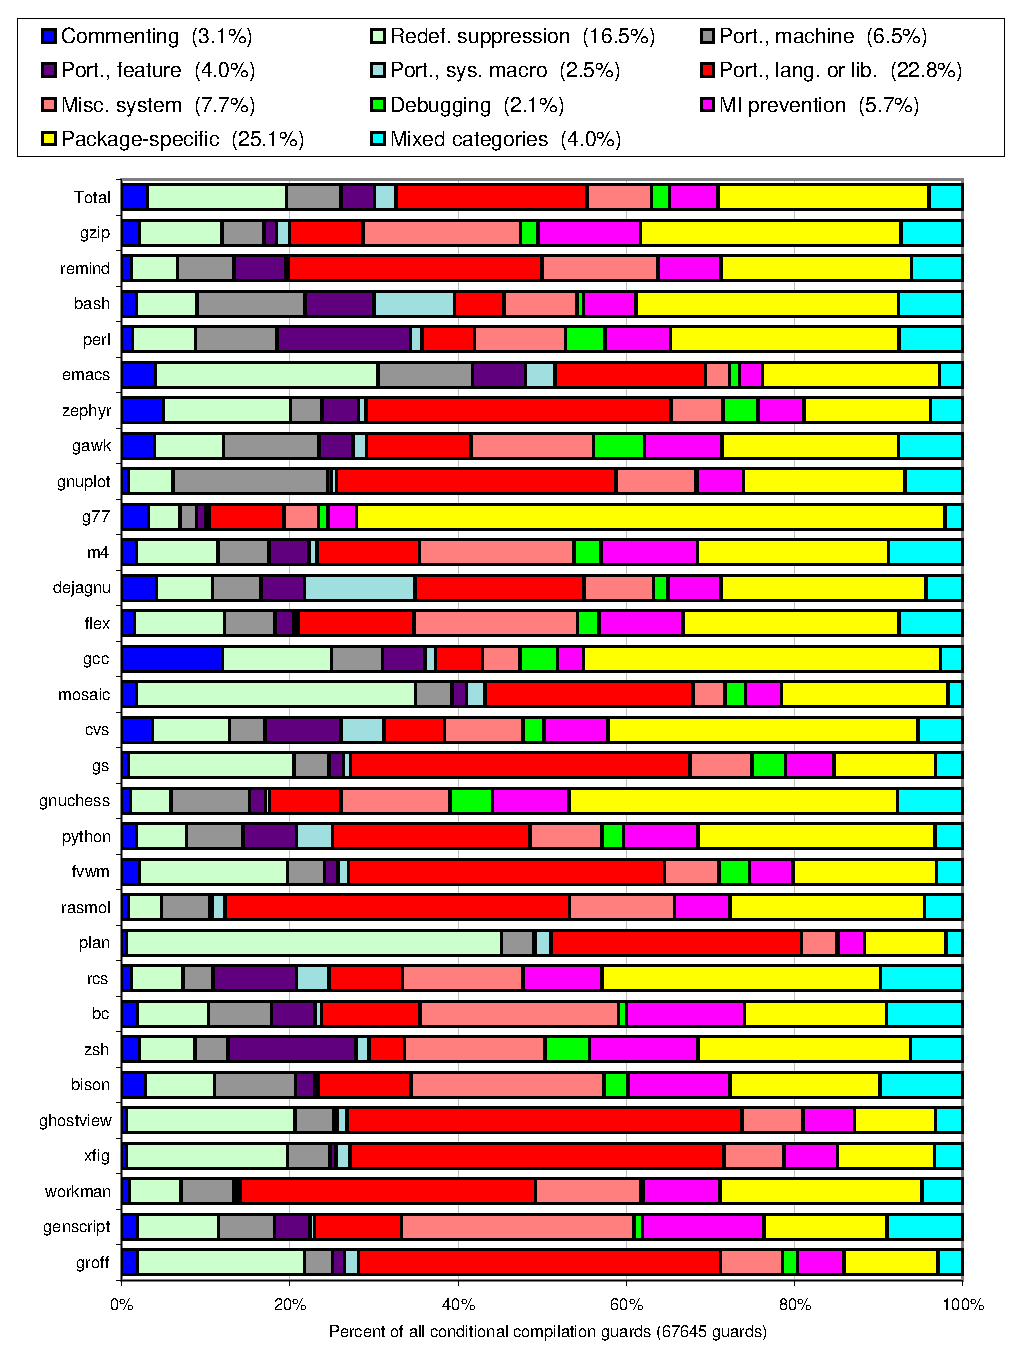
\epsfig{file=fig/ccd-categories.eps,height=6in}}
\centerline{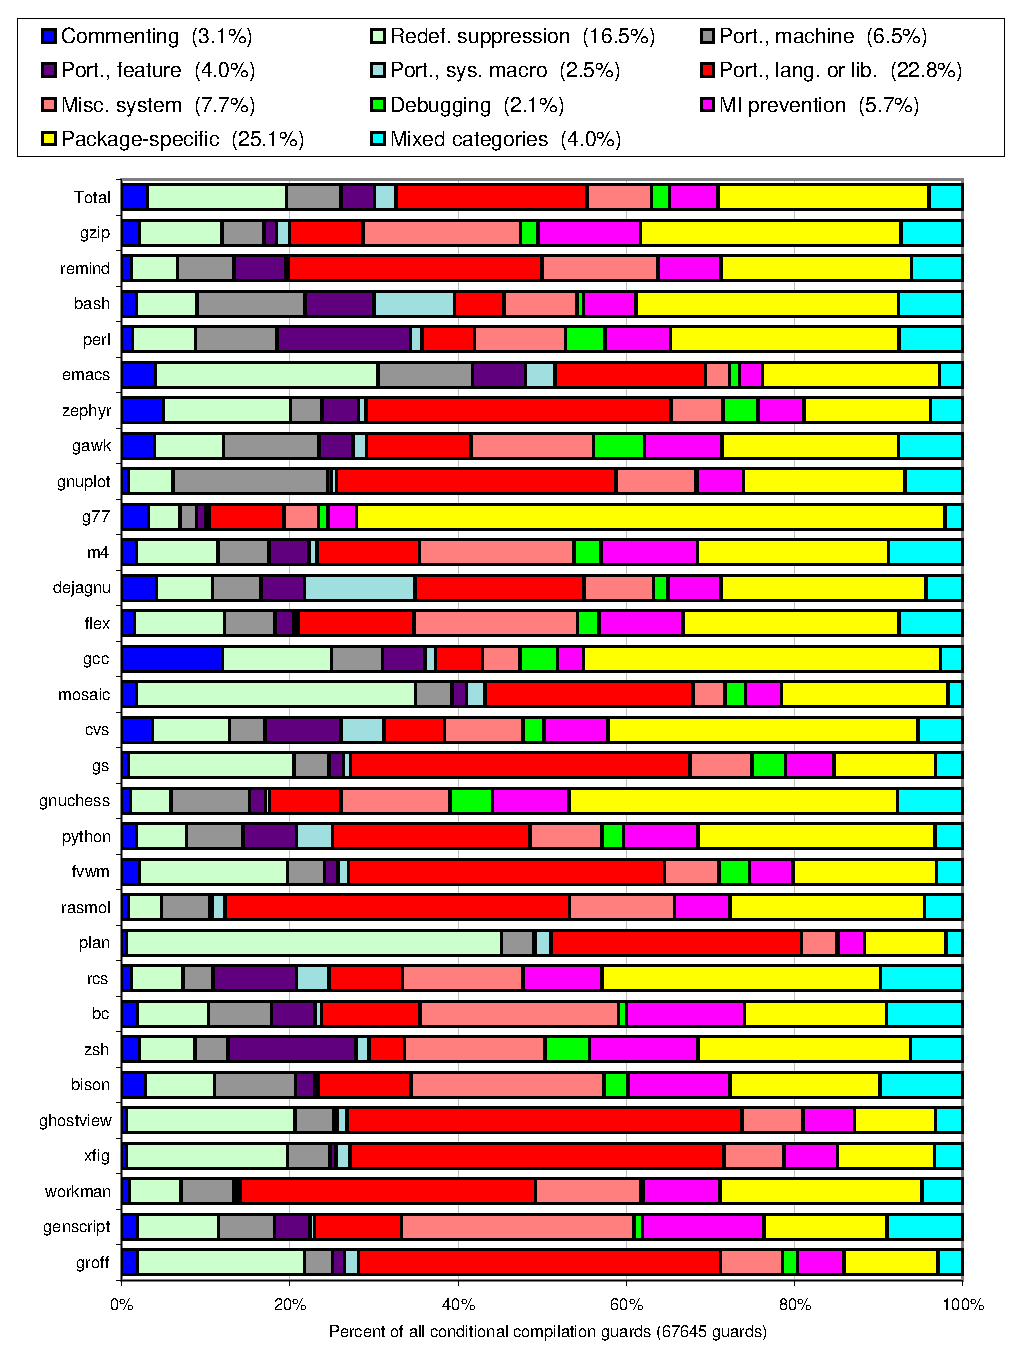
\epsfig{file=fig/ccd-categories.eps,angle=270,width=\linewidth}}
\captionsmall{Purposes for conditional compilation directives.
  The legend indicates what percentage of all Cpp conditionals fall
  into each category, numerically presenting the information in the top row
  of the chart.}
\label{fig:ccd-categories}
\end{figure}

Cpp conditionals are used to control inclusion of code for portability,
debugging, efficiency, and other purposes.  The programmer intention behind
a {\tt \#if} line can often be inferred from its structure, its context, or
the purpose of the macros it uses.

% This classification can reveal the structure of
% conditional compilation directives and assist in program understanding.

Figure~\ref{fig:ccd-categories} shows the heuristically determined purpose
of each Cpp conditional in our test suite.  First, the heuristic classified
some conditionals according to their structure or context, as follows:
\begin{description}\itemsep 0pt \parskip 0pt
\item[Commenting] These guards either definitely succeed and
  have no effect as written (e.g., \texttt{\#if 1}), or definitely fail
  and unconditionally skip a block (e.g., {\tt \#if (0 \&\&
  \verb|OTHER_TEST|)}).  These guards comment out code or override other
  conditions (e.g., to unconditionally enable or disable a previously
  experimental feature).
      
\item[Redefinition suppression] These guards test non-definedness of
  symbol, and control only a definition of the same symbol, thus avoiding
  preprocessor warnings about a redefinition of a name (e.g.,
  \texttt{\#ifndef FOO} followed by \texttt{\#define FOO ...} and
  \texttt{\#endif}).  
  The purpose is to provide a default value used unless another part of the
  system, or the compilation command, specifies another value.

\end{description}

For Cpp conditionals not classified by the above rules, the purpose of each
macro name appearing in the conditional is determined from the system
properties it reifies.  If each macro in the conditional has the same
purpose, then the conditional is given that purpose; otherwise, the
conditional is classified as ``mixed usage''.  The macro purposes, which
are determined from the macro's name rather than an examination of its
definitions (which are often either unavailable or trivial, such as the
constant {\tt 1}), are as follows:

\begin{description}\itemsep 0pt \parskip 0pt
%% See ccd_lexical_category in em_analyze for the routines
%% which implements these heuristics

\item[Portability, machine]
  These symbols name the operating system or machine
  hardware (e.g., \texttt{sun386} or \texttt{MACINTOSH}).
      
\item[Portability, feature] These symbols describe specific parameters
      or capabilities of the target machine or operating system (e.g.,
      \texttt{BYTEORDER}, \verb|BROKEN_TIOCGWINSZ|).  
      
%      These symbols are different from ``portability, machine'' because
%      they may correspond to multiple machines or architectures.

\item[Portability, system]
  These symbols are commonly defined constants or
  pseudo-inline functions in system or language libraries (e.g.,
  \verb|O_CREATE|, \texttt{isalnum}, \verb|S_IRWXUSR|).

\item[Portability, language or library]
  These symbols are predefined by a compiler, defined by a standard
  library, or defined by the package as part of the build
  process to indicate existence of compiler, language, or library features
  (e.g., \texttt{GNUC}, \texttt{STDC}, \verb|HAS_BOOL|).

\item[Miscellaneous system]
  These symbols are reserved (they begin with two underscores) and do
  not fit any other purpose.
      
\item[Debugging]
  These symbols control inclusion of debugging or tracing code.  The macro
  names contain \texttt{DEBUG} or \texttt{TRACE} as substrings.
      
\item[Multiple inclusion prevention]
  These guards encompass an entire file to ensure that the enclosed code is
  seen only once per translation unit by the compiler.  Such guards are
  indicated by convention with a trailing \verb|_H| or \verb|_INCLUDED| in the macro name
  they check.

\item[Package-specific] 
  These symbols are specific to the given package.  They do not fit any of
  the other purposes.

\item[Mixed usage] These guards test multiple symbols
  that have different purposes (e.g., {\tt \#if defined(\verb|STDIO_H|) ||
  \verb|SYSV_SIGNALS|}).

\end{description}


%%Numbers: read off legend of fig/ccd-categories.eps

There is significant variation among packages, and no clear pattern of use
emerges.  Portability accounts for 37\% of conditional compilation
directives.  Redefinition warning suppression, at 17\%, is surprisingly
high; it is essentially a macro definition mechanism, not a conditional
inclusion technique.  Mixed usage is relatively rare.  This suggests both
that the conventions for macro names are fairly standardized and that
programmers rarely write conditional tests that combine entirely different
concerns in a single expression.

%%Numbers:
%% 23% = fig/ccd-categories.eps: ``redef. suppression'' + ``MI prevention''
%% 37% = fig/ccd-categories.eps: ``port., *''

These data suggest that 23\% of conditional compilation directives
would be unnecessary if the C preprocessor had two simple language
features: a ``define only if not already defined'' directive and 
an Objective-C-like \ppd{import} facility which automatically avoids
multiple inclusions.  Another 37\% of conditional compilation directives
involve variances in target operating
systems.  Tools such as the GNU project's \texttt{autoconf} may account
for the prevalence of these guards by making it easier to maintain code
bases with sprinkled \ppd{ifdef}s managing multiple target operating
system variants.  It would be interesting to compare these data to those
collected for software that targets only a single specific platform.

% \subsection{Number of arguments}
% 
% \begin{figure}
% \centerline{\epsfig{file=fig/cat-numargs.eps,height=4in}}
% \captionsmall{Is this worth including?
%   [[PROBLEM:  the numbers in this legend do not accord with those in
%   previous legends by name.  This is because the numargs information was
%   gleaned from the .catg file which contains only the macro bodies and
%   the filename they were found in, thus there is no way to include macro
%   bodies defined outside the package of macro names that are defined
%   somewhere inside the package as is the case almost everywhere else;
%   I am now thinking that this information could/should have been used
%   for aiding the categorizations: i.e., a null define taking no
%   arguments is a lot different than one taking arguments;  since that
%   was not done, I am inclined to drop this since to avoid the
%   inconsistency in the numbers (and because it is of questionable
%   utility as presented now --gjb]]}
% \label{fig:cat-numargs}
% \end{figure}
% 
% 
% You might wonder whether macros are used like functions (taking arguments)
% or like constants (taking no arguments).  
% [[However, a fair number of statement macros also take no arguments.]]
% We graphed that in
% Figure~\ref{fig:cat-numargs}.  This seems irrelevant to me; I do not see
% where to fit it in, or what to say about it.



\section{Dependences}
\label{sec:dependence}
\label{sec:last-content-section}

Macros control the program that results from running Cpp via inclusion
dependences and expansion dependences.  This section reports the incidence
of these dependences, both by macro and by line.

\emph{Inclusion} dependence results from Cpp conditionals that test macros
to determine which lines of the Cpp input appear in the output.  A line is
inclusion-dependent on a macro name if and only if the macro's definedness
or its expansion can affect whether the line appears in the preprocessor
output.  In other words, there is a set of values for all other macros such
that the line appears in the output for one value of the macro (or for the
case of the macro being undefined) and does not appear in the output for
the other value of the macro (or for the case of the macro being
undefined).  This notion is related to control dependence in program
analysis.

\emph{Expansion} dependence results from replacement of macros outside Cpp
conditionals by their definition bodies, which controls the content of the
lines on which the macros appear.  A line is expansion-dependent on a macro
name if the macro's definedness or value affects the text of the line after
preprocessing.  In other words, for some set of values for all other
macros, setting the macro to one value (or undefining it) results in a
different final text for the line than setting the macro to a different
value (or undefining it).  This notion is related to data dependence in
program analysis.

We report both direct and indirect dependences.  A line directly depends
upon macros that appear in the line or in a {\tt \#if} condition whose
scope contains the line.  It indirectly depends on macros that control the
definitions of directly controlling macros.  After {\tt \#define
\verb|S_ISBLK|(m) ((m)~\&~\verb|S_IFBLK|)}, the final text of a line that
uses \verb|S_ISBLK| depends not just on its definition but also on that of
\verb|S_IFBLK|.  An indirect dependence is an expansion dependence if every
dependence in the chain is an expansion dependence; otherwise, the indirect
dependence is an inclusion dependence.

We distinguish \emph{must} from \emph{may} dependences.  A must dependence
links a use to the macro's known single definition site; a may dependence
links a use to multiple definition sites, when it is not known which
definition is in effect at the point of use.  When a macro is defined on
both branches of a {\tt \#if} conditional, the macro's definedness does not
depend on the values tested in the conditional, though its value might.  We
do track dependences across file boundaries: if a macro controls whether a
file is {\tt \#include}d, then the macro also controls every line of that
file.

%% This makes absolutely no sense.  What is going on here?
%% I think there's something meaningful about lopping off prefixes of must
%% dependences, but cannot puzzle it out now.  -MDE 11/1/97
% When different conditions control different definitions of a macro, uses
% are dependent on the independent parts of those conditions.  For instance,
% after
% \begin{verbatim}
%   #if A
%     #if B1
%       #define M ...
%     #elsif B2
%       #define M ...
%     #else
%       #define M ...
%     #endif
%   #endif
% \end{verbatim}
% a use of macro {\tt M} is expansion-dependent on {\tt B1} and {\tt B2}, but
% not on {\tt A}, which must have been set to true in order for {\tt M} to be
% defined at all.  That is, no setting of {\tt A} can affect {\tt M}'s

The statistics reported in this section are underestimates because they
omit \pkg{emacs}, which aggressively uses macros.  Its full dependence
information exceeded 512 MB of virtual memory, in part due to its optional use of Motif,
a complex external library with extensive header files.  (While this paper reports only on macros
defined in each package, we computed dependences and other information for
all macros, including those defined or used in libraries.  Additionally,
our implementation is not optimized for space.)  We did generate dependence
information for \pkg{mosaic} and \pkg{plan}, which also use Motif.


\subsection{Dependences by line}

\begin{figure}
\centerline{\epsfig{file=fig/dep-byline.eps,height=4in}}
%%Numbers: read off Excel dep-byline
\captionsmall{Percentage of lines dependent on a particular number of macros (or
  fewer).  For instance, 94\% of all lines are expansion-dependent on 2
  or fewer macros, and 90\% of all lines are inclusion-dependent on 10 or
  fewer macros.  Lines higher in the graph indicate dependence on fewer
  macros.  The values for 0 macros (which does not fall on the log-scale x
  axis) are as follows:  75\% of lines expand no macros, 63\% of lines are
  unconditionally included (or excluded), and 60\% of lines are not
  dependent on any macros at all.}
\label{fig:dep-byline}
\end{figure}

%%Numbers: read off Excel dep-byline

%%Numbers: Weighted averages of tbl-dep-byline = (8.23 0.5854 8.70)

Figure~\ref{fig:dep-byline} graphs the percentage of lines dependent on a
given number of macros.  On average, each line in the {\numdependpackages}
packages we did dependency analysis on is expansion-dependent on 0.59 macros, inclusion-dependent
on 8.2 macros, and has some dependence on 8.7 macros.  Some lines that are
inclusion-controlled by macros do appear unconditionally in the package
source but are inside a guard to avoid multiple inclusion\,---\,this is the
case for many header files.

%%Numbers: read off Excel dep-byline

Expansion dependence on multiple macros is not prevalent\,---\,only 3.6\% of
lines are expansion-dependent on more than 3 macros, and only 1.1\% are
expansion-dependent on more than 7 macros.  However, one line of
\pkg{gcc}\,---\,{\tt \verb|LEGITIMIZE_ADDRESS| (x, oldx, mode,
win);}\,---\,is expansion-dependent on 41 different macros.  (When we
examined all source code, not just one architecture/operating system configuration, it
was expansion-dependent on 187 macros!)  Macro \verb|LEGITIMIZE_ADDRESS|, which
creates a valid memory address for a memory operand of a given mode,
is defined 30 times in \pkg{gcc}, with many of the definitions dozens of
lines long and themselves studded with macro invocations.
Inclusion dependences have a much wider distribution.  Overall, 10\% of lines
are inclusion-dependent on at least 10 macros, and 1\% of lines are
dependent on over 176 macros.

%   \comment{check
%   these numbers; where did I get them?}Overall, only 13 out of
% 325,000\comment{be specific?} lines in \pkg{gcc}\comment{what about
%   elsewhere?} are expansion-dependent on more than 100 macros.

% \comment{double-check these numbers; I think
% em_analyze -L does that.}As an example, the line of \pkg{gcc}
% mentioned above has 182 inclusion dependences (with only 13 macros in
% common with its set of expansion dependences), but over 10,000 lines
% of \pkg{gcc} have even heavier inclusion dependences than that.

\subsection{Dependences by macro}

\begin{figure}
% This works, but the figures are upside-down.
% \centerline{\epsfig{file=fig/exp-dep-bymacro.eps,angle=90,height=3.75in}}
% \centerline{\epsfig{file=fig/incl-dep-bymacro.eps,angle=90,height=3.75in}}
% Cannot use ``height'' when rotating by -90 or +270; I do not know why.
% \centerline{\epsfig{file=fig/exp-dep-bymacro.eps,angle=270,width=.5\linewidth}}
% \bigskip
% \centerline{\epsfig{file=fig/incl-dep-bymacro.eps,angle=270,width=.5\linewidth}}
% When Mike exports Excel charts, angle is 270.  When Greg exports, angle is 0.
\centerline{\epsfig{file=fig/exp-dep-bymacro.eps,angle=270,width=.48\linewidth}%
\ %
\epsfig{file=fig/incl-dep-bymacro.eps,angle=270,width=.48\linewidth}}
%%Numbers: read off of Excel exp-dep-bymacro
\captionsmall{Dependences by macro name for \numdependmacronames\ macro
  names in \numdependpackages\ packages.  Each bar represents all macros
  that control at least as many as the labeled percent of the lines in its
  package (but fewer than the next bar).  For instance, the 0.17 bar in the
  expansion dependence chart indicates that 257 macros each control between
  0.17\% and 0.26\% of the entire package that contains that macro.  The
  maximum falls in the penultimate bucket (i.e., the rightmost bucket is
  the first empty one).  The $\varepsilon$ bar represents a small non-zero
  fraction (specifically, $10^{-7}$), so that macros not controlling any lines
  are not conflated with macros controlling very few lines.  A log scale is
  used for the x axis.}

%% expansion is red; inclusion is blue
\label{fig:dep-bymacro}
\end{figure}

Figure~\ref{fig:dep-bymacro} graphs how many lines are dependent on each
macro (Figure~\ref{fig:dep-byline} gave the same information by line rather
than by macro).  Since the {\numdependpackages} packages vary in size, the
graphs of Figure~\ref{fig:dep-bymacro} aggregate them by reporting
percentages of a package rather than absolute numbers.

%% The second sentence of this paragraph is a non sequitur.

%%Numbers: 2.0% = half of the ``conditional'' bar of Excel directives-breakdown

%% This doesn't approximate Zipf's law when using ranking numbers; I extracted
%% the non-zero numbers from tbl-any-dependences-by-macro, then did:
% (while (not (eobp))
%   (let ((val (* (1+ (count-lines 1 (point)))
%               (string-to-number (buffer-substring
%                                    (point)
%                                    (progn (end-of-line) (point)))))))
%     (insert "\t" (number-to-string val))
%     (forward-line)))
%% but looking at the data in the chart, we can multiply percents times
%% frequencies to get something nearly constant, except at the edges.

The expansion dependence chart illustrates that most macros control few
lines, a few macros control many lines, and the transition between the two
varieties is gradual.  (The values follow a variant of Zipf's
law~\cite{Zipf49}:  the product of the number of macros and the percentage
of lines dependent on those macros is nearly constant.  Excluding the first
four and last two buckets, which represent extremal values, the
product's average is 40, with a standard deviation of 8.7.)  Most {\tt
\#if} directives (which account for 2.0\% of all lines) expand at
least one macro; the rare exceptions include testing the compiling
machine's character set.

%%Numbers:  Find the highest numbers in tbl-expansion-dependences-by-macro.
%% Determine the packages containing them.
%% In the sdepend files for those packages, and find the highest line counts:
%%  (delete-non-matching-lines "\\+ [0-9][0-9][0-9][0-9])")
%% or   egrep '\+ [0-9][0-9][0-9][0-9]' *.sdepend

%% 5.1613       cvs     NULL    constant
%% 4.1558       gcc     rtx     type
%% 4.1285       genscript       AFM_ENC_NONE    constant
%% 4.9994       gs      const   type
%% 4.2015       mosaic  NULL    constant
%% 5.2562       perl    SvANY   type
%% 4.302        rcs     const   type
%% 5.2813       xfig    ArgCount        check dynamic binding
%% 5.2401       xfig    Args    check dynamic binding
%% 
%% 3.4216       bash    ISFUNC  sometimes constant, sometimes function expression
%% 3.4485       gawk    NULL    constant
%% 3.240        gnuplot fprintf function
%% 3.4733       m4      NULL    constant
%% 3.8026       perl    void    type
%% 3.7568       perl    curinterp       variable renaming
%% 3.0103       perl    op      variable renaming
%% 3.7546       rasmol  __far   type
%% 
%% ;; round out the top 20
%% 2.9615       fvwm    NULL    constant
%% 2.959        gs      private_        type
%% 2.9888       gzip    local   type
%% 2.9661       perl    SvFLAGS expression
%% 2.9751       rcs     P       type declaration
%% 
%% ;; One more very close to those.
%% 2.9575       gs      private type


%% 5.2813       xfig    ArgCount        manage dynamic binding
%% 5.2401       xfig    Args    manage dynamic binding
%% 3.7568       perl    curinterp       variable renaming
%% 3.0103       perl    op      variable renaming
%
%% 4.1558       gcc     rtx     type
%% 5.2562       perl    SvANY   type
%% 2.959        gs      private_        type
%% 2.9888       gzip    local   type
%% 2.9751       rcs     P       type declaration
%
%% 4.1285       genscript       AFM_ENC_NONE    constant
%% 2.9661       perl    SvFLAGS expression
%% 3.4216       bash    ISFUNC  sometimes constant, sometimes function expression
%
%% 3.240        gnuplot fprintf function (provide specialized version)
%% 3.7546       rasmol  __far   type
%% 4.9994       gs      const   type
%% 4.302        rcs     const   type
%% 3.8026       perl    void    type
%% 5.1613       cvs     NULL    constant
%% 2.9615       fvwm    NULL    constant
%% 3.4485       gawk    NULL    constant
%% 3.4733       m4      NULL    constant
%% 4.2015       mosaic  NULL    constant


Each of the 20 most frequently used macros is expanded on at least 3.0\% of
lines in its package.  Four of these (in \pkg{xfig} and \pkg{perl}) rename
variables to manage dynamic binding or linking.  Two are user-defined types
({\tt rtx} in \pkg{gcc} and {\tt SvANY} in \pkg{perl}), two are user-defined
type modifiers (\verb|private_| in \pkg{gs} and \verb|local| in
\pkg{gzip}), and one creates either ANSI or K\&R function prototypes ({\tt
P} in \pkg{rcs}).  One is a user-defined constant (\verb|AFM_ENC_NONE| in
\pkg{genscript}), another is an expression ({\tt SvFLAGS} in \pkg{perl}),
and another is incompatibly defined sometimes as a constant taking no
arguments and sometimes as an expression taking arguments ({\tt ISFUNC} in
\pkg{bash}).  The other ten redefine built-in quantities:  {\tt fprintf} in
\pkg{gnuplot} to substitute a custom version, \verb|__far| in \pkg{rasmol}
because that is meaningful only in x86 dialects of C, and {\tt void} in
\pkg{perl}, {\tt const} in \pkg{gs} and \pkg{rcs}, and {\tt NULL} in
\pkg{cvs}, \pkg{fvwm}, \pkg{gawk}, \pkg{m4}, and \pkg{mosaic}.  
Because we determined which symbols are macros by running a modified
version of the preprocessor, we report such redefinitions only when the
package may override the built-in version.  Generally, only a few such
built-in symbols are overridden.


The inclusion dependence graph is bimodal.  While most macros control
inclusion of zero or few lines, quite a few control over 5\% of the
package, and there are not a lot of macros in between.  The graphs for the
individual packages exhibit far higher peaks than the aggregate inclusion
dependence graph of Figure~\ref{fig:dep-bymacro}; summing the graphs tended
to average them.  The heaviest dependences tend to be on macros controlling
header file inclusion.

%%  (for
%% instance, \verb|H_PERL| controls inclusion of over 53\% of \pkg{perl}'s
%% lines).\comment{How does it look if we separate these out?}

%        [[It would have been interesting to run these numbers for everything
%          but exclude file multiple inclusion prevention macros.]]


\subsection{Cpp partial evaluation}

% These define __P:  grep __P *.catg
%   bash cvs emacs gcc gs m4 rcs zephyr
% These use __P:  grep ": __P," `findfile expansions.lst`
%   (delete-non-matching-lines "expansions.lst:\\.")
%   bash emacs zephyr
% Uses __PROTO:  cvs
% Partially uses HAVE_PROTOTYPES: xfig
% Partially uses proto: perl
% Partially uses __STDC__: mosaic, bison
% Partially uses NeedFunctionPrototypes: ghostview
% Uses HAVE_PROTOS:  remind
% Uses PROTOTYPES and _: m4
% Uses HEADERS:
% Uses FUNCPROTO (but only for wholesale inclusion/exclusion): rasmol
% Uses OF: gzip
% Uses P: gawk
% Uses DC_DECLARG: bc
% Uses ARGS[1-9]: mosaic

% A = ANSI only
% K = K&R only
% B = both
% S = primarily one dialect, but some code does both

% B bash-1.14.7
% B bc-1.03
% S bison-1.25
% B cvs-1.9
% B emacs-19.34
% K flex-2.5.4
% A fvwm-2.0.43
% B gawk-2.15.6
% B gcc-2.7.2.3
% A genscript-1.3.2a
% S ghostview-1.5
% A gnuchess-4.0.pl77
% K gnuplot-3.50.1.17
% B gs-5.10
% B gzip-1.2.4
% B m4-1.4
% S mosaic-2.6
% S perl-5.003
% K plan-1.7.1
% B rasmol-2.5
% B rcs-5.7
% B remind-03.00.16
% K workman-1.3
% S xfig-3.1.4
% B zephyr-2.0.4
% S zsh-3.0.5
%
% I think workman was the only package which saw no code size reduction.

Support for multiple dialects of a language, such as ANSI~C and K\&R~C, is
a common use of the preprocessor:  3 of the {\numpackages} packages support
only ANSI~C, 4 support only K\&R~C, 13 use the preprocessor to fully
support both dialects, and 6 prefer one dialect but partially support
another (for instance, part of the package supports both dialects or a
substantial number of functions have both varieties of prototype).  Such
support is possible only in the preprocessor, not in the language, and
leads to unstructured macros (partial declarations and other
difficult-to-handle constructs).  Furthermore, these uses are highly
visible and distracting to programmers and tools, because they may change
the syntax of every function declaration and definition.

%% I found these uses by doing:
%% search -i -n '[^-a-zA-z0-9_](__P|__proto|__PROTO|proto|PROTO|_|OF|P) *\(.*[^;\n]$'

%% This looks like a partial discussion to me; could show several
%% approaches, but probably not worth the ink.
% One approach is to supply different headers for the two C dialects, as in
% \pkg{remind}:
% {\small
% \begin{verbatim}
%     #ifdef HAVE_PROTOS
%     PRIVATE void PrintLeft(char *s, int width, char pad)
%     #else
%     static void PrintLeft(s, width, pad)
%     char *s; int width; char pad;
%     #endif
%     { ... }
% \end{verbatim}
% }

We performed an experiment to determine whether eliminating these macros
would simplify understanding or analysis by reducing the complexity of
macro definitions and usage as measured in this \typeofdocument.  We built
a Cpp partial evaluator called Cppp.  Given Cpp-style command-line
arguments specifying which macros are known to be defined or undefined
(and, optionally, their expansions), Cppp discharges Cpp conditionals,
including nested conditionals, that depend on those macros.  Other
conditionals, and macro uses, remain in the output.  Cppp does not expand
macros inline or use macro definitions found in its input files.  Cppp is
similar to the {\tt unifdef} program distributed with some Unix variants,
except that {\tt unifdef} does not
permit specifying a value for a defined symbol and only operates on {\tt
\#ifdef} tests.

% (It does not eliminate or expand other macros with only one
% remaining definition, because other definitions may appear in libraries or
% on the command line when the package is compiled.)

% computed 1/28/99: I got the raw data to compute the 1.2% figure by doing
%   foreach PACK ($PKG_DIRS)
%      echo $PACK; cd /scratch/mernst/pack-cppp/$PACK; wc `grep -v '^#' c-files-listing` | tail -1
%   end
% and likewise for /scratch/mernst/packages

% \comment{Uses per line dropped from .31
% to .28 with pcp3; but we also changed which files we were examining...}

We used Cppp to preprocess all of our test suite (and all library header
files) with definitions for all the macros that can be depended on if using
ANSI standard C or C++ (including prototypes and booleans) and
POSIX-compliant libraries.  This reduced the size of the codebase by 1.2\%
overall; individual package reductions ranged from 3.2\% for \pkg{emacs} to
none at all for \pkg{workman}.  We then reran all of our experiments, but
to our surprise, the results were little changed from the full versions of
the packages.  The decline in multiple definitions of macros, ``other''
categorizations, dependences on macros, and other metrics we report were
single-digit percentages of their original values.  We conclude that
extra-linguistic macro usage in our test programs presents no obvious
single point of attack:  even eliminating one highly prevalent and visible
use\,---\,which was also the largest identifiable source of Cpp
conditionals (see Figure~\ref{fig:ccd-categories})\,---\,did not
significantly reduce the complexity introduced by preprocessor.

Discharging selected conditionals can sometimes be worthwhile, however.
The developers of the \pkg{Scwm} window manager~\cite{Scwm} used our Cppp tool to eliminate
numerous compile-time options inherited from \pkg{Scwm}'s predecessor,
\pkg{fvwm2}.  This transformation resulted in a cleaner code base that the
developers found easier to understand and modify.



\section{Related work}
\label{sec:related}

We know of no other empirical study of the use of the C preprocessor nor
any other macro processor.  However, the literature does contain guidance on
using C macros effectively and on writing portable code, tools for checking macro usage, and techniques
for understanding and exploring C source code that uses the preprocessor.

\subsection{Style guidelines}

Several coding style guides make recommendations on preprocessor use and on
ways to reduce unexpected behavior resulting from poorly designed
constructs~\cite{Cannon90}.  Our empirical data help refine these sets of
suggestions, both by extending their taxonomies and recommendations and by
indicating which problems occur in practice.

The GNU C preprocessor manual~\cite{cpp-manual} discusses
a set of techniques including simple macros, argument macros, predefined
macros, stringization macros, concatenation macros, and undefining and
redefining macros.  Its list of ``pitfalls and subtleties of macros'' include
unmatched parentheses, unparenthesized formals and bodies, dangling
semicolons, multiple formal uses, and self-referential macros.  It also
discusses three issues not addressed in this paper:  argument prescan
(macro arguments are actually scanned for macro expansions twice), cascaded
macros (macro bodies use the current definition of other macro, not the
ones in effect at the definition site), and newlines in macro invocations
(which can throw off error line reporting).

The GNU coding standards~\cite{Stallman97} mention Cpp only to recommend
upper case for macros and use of macros to provide meanings for standard
symbols on platforms that don't support ANSI~C\@.
The Ellemtel coding standards~\cite{ellemtel92} recommend that inline
definitions appear in separate files of their own (not in \file{.h} header
files) that never include other files, that inline functions and {\tt
const} or {\tt enum} constants be used in place of {\tt \#define}, and that
preprocessor macro names be prefixed to avoid name clashes.

An adaptation of the Indian Hill C Style and Coding
Standards~\cite{Cannon90} makes numerous suggestions. Programmers should use all capital letters for macro
names except for macros that behave like function calls, which are
acceptable only for short functions.  Statement macros should be wrapped in
{\tt do \{ \ldots{} \} while (0)}, particularly when they contain keywords.
Conditional bodies should be fully bracketed to avoid dangling semicolons.
Macros should evaluate their parameters exactly once and arguments should
not have side effects.  Side effects to macro parameters should be
documented.  Macros should avoid using global variables, since the global name may
be hidden by a local declaration.  Macros with bodies that are long or
that reference variables should take an empty parameter list.  Programmers
should use the ANSI specification rather than preprocessor tricks such as
using {\tt /**/} for token pasting and macros that rely on argument string
expansion.  Syntax should not be changed by macro substitution (except for
the {\tt PROTO} macro).  While {\tt \#ifdef} is to be avoided, it should
appear in header files (which should not be nested) rather than source
code.  It can be used to protect {\tt \#pragma} and to define macros that
are used uniformly in the code, without need for further {\tt \#ifdef}.  If
a machine is not specified, compilation should fail rather than using a
default; but conditional compilation should generally test features, not
machines or operating systems.  The text inside an {\tt \#ifdef}-bracketed section
should be parsable code, not arbitrary text.

Stroustrup~\cite{Stroustrup-DesignEvolution} lists 14 tasks supported by
the C preprocessor and notes C++ alternatives for 5 of the 8 uses of {\tt
\#define}:  constants, inline subroutines, parameterized types and
functions, and renaming.  While a principle of C++'s design was elimination
of the preprocessor, C++ continues to rely on it for the other uses
Stroustrup lists:  {\tt \#define} for string concatenation, new syntax, and
macro processing, {\tt \#ifdef} for version control and commenting, {\tt
\#pragma} for layout and control flow hints (though pragmas are
disparaged), and {\tt \#include} for exporting declarations and composing
source text.  Stroustrup proposes moving {\tt \#include} into the language,
which could eliminate some of its quirks and simplify the task of
programmers and tool writers, as the {\tt \#import} directive does for
Objective-C~\cite{CoxN91}.  Stroustrup remarks that ``In retrospect,
perhaps the worst aspect of Cpp is that it has stifled the development of
programming environments for C.''

Carroll and Ellis~\cite{Carroll95} list eight varieties of non-{\tt
\#include} macro usage, culled in part from Stroustrup's
list~\cite{Stroustrup-DesignEvolution}.  They say that C++ can replace
these uses of the preprocessor other than declaration macros (such as
declaring a class constructor and destructor via a macro call) and code
versioning (such as debugging versions).  They also recommend the use of
corporation- and project-specific prefixes to avoid macro name and header
file name conflicts.


\subsection{Portability}

Two other style guidelines focus on portability concerns.
Dolenc et al.~\cite{Dolenc90} warn of implementation limits permitted by the C language standard such
as 32~nesting levels of parenthesized expressions, 1024~macro identifiers,
and 509~characters in a logical source line.  They also note
incompatibilities among preprocessors that usually result from failure of
implementations to conform to the specification.  For instance, some
non-standard preprocessors do not support the {\tt defined} operator or the {\tt
\#pragma} or {\tt \#elif} directives, ignore text after the {\tt
\#else}, {\tt \#elif}, and {\tt \#endif} directives, or perform
concatenation and stringization in nonstandard orders during macro
substitution.  The authors recommend using some of these
incompatibilities\,---\,such as accepting only directives starting in the
first column, without leading whitespace\,---\,along with {\tt \#ifdef} to
hide modern Cpp features from older preprocessors.  The paper also treats
in detail specific header files that may cause portability problems,
showing how to overcome these difficulties, generally by using
the macro preprocessor to define some symbols (more) correctly.


Spencer and Collyer~\cite{SpencerC92} provide a set of techniques for
achieving portability without using \texttt{\#ifdef}, which they recommend
only for providing default values for macros and preventing multiple
inclusion of header files.  The paper is as much about good software
engineering as it is about the preprocessor per se, but does
contain some preprocessor-specific recommendations.  The authors suggest using
standard interfaces, then providing multiple implementations if necessary.
These implementations should appear in separate files rather than sharing
code via {\tt \#ifdef}, and the build or configure script should select
among them; thus, a choice of files replaces Cpp conditionals.  An override
directory early in the search path permits bad include files to be replaced
rather than selectively overridden.  More uses of {\tt \#ifdef} can be
eliminated by moving system-specific tests and operations into shell
scripts or by using standard programs (such as {\sf ls} or {\sf df})
instead of accessing system services from C code.  (These strategies can
complicate porting to non-Unix systems, and even standard programs may have
different behavior in different places.)  Use of the preprocessor to
establish numeric constants should be viewed with suspicion;
dynamically-sized objects are a better approach.  Uses of {\tt \#ifdef}
should test for features or characteristics, not machines, and an error is
desirable to selecting a default machine.  Spencer and Collier recommend
that {\tt \#ifdef} be restricted to declarations and macro definitions,
never used at call sites, and that {\tt \#include} never appear inside {\tt
\#ifdef}.  They also break down the uses of \texttt{\#ifdef}
in the 20,717 lines of their C News program.  Of the 166 uses, 36\% protected a default
value for a preprocessor symbol, 34\% were used for configuration, 15\%
commented out code, and 3\% prevented multiple inclusion of header files.


\subsection{Error checking}

Krone and Snelting use mathematical concept analysis to determine the
conditional compilation structure of code~\cite{Krone94}.  They determine
the preprocessor macros each line depends upon (in our terminology, they
only compute inclusion dependence, not expansion dependence) and display
that information in a concept lattice.  They do not determine macro
relationships directly, but only by their nesting in {\tt \#if}, and
the information conveyed is about the program as a whole.  Each point in
the lattice stands for a set of lines dependent on exactly the same
preprocessor symbols, though not necessarily in exactly the same way.  The
lattice can reveal that one macro is only tested within another one's
influence, for example.  When the lattice does not have a regular grid-like
structure, it is possible that the code does not properly separate
concerns.  The most closely related part of our paper is
Section~\ref{sec:ccd}, which analyzed single compilation directives that
tested multiple incompatible macros using a fixed set of macro purposes.


%Greg:  describe LCLint methodology and results.  Say exactly what you did
%(i.e., how hard you tried), and what the results were.  Also, that you tried
%on only 20, not all 30, packages, which does not include the biggest ones.

A number of tools check whether specific C programs satisfy particular
constraints.  Various lint~\cite{Johnson77} source-code analyzers check for
potentially problematic uses of C, often including the C preprocessor.
Macro errors are usually discovered as a byproduct of macro
expansion\,---\,for instance, by generating an empty statement that causes
lint to issue a warning\,---\,rather than in their own right.  A survey of
nine C++ static checkers~\cite{MeyersK97} mentions the macro preprocessor only
in terms of whether such warnings can be turned off in the tools; however,
that paper focuses on coding style likely to lead to errors rather than on
lexical issues.


%%Numbers: 3184 parse errors, 571 internal bugs, 4069 files = 92% failure rate

LCLint~\cite{Evans-fse94,Evans:LCLint} allows the programmer to add
annotations that enable more sophisticated checks than many other lint
programs.  LCLint optionally checks function-like macros\,---\,that is,
those that take arguments\,---\,for macro arguments on the left hand side
of assignments, for statements playing the role of expressions, and for
consistent return types.  LCLint's approach is prescriptive:  programmers
are encouraged not to use constructs that might be dangerous, or to change
code that contains such constructs.  For full checking, LCLint also
requires users to add fine-grained annotations to macro definitions.  We
tried to run LCLint version 2.3i on our set of packages with its macro diagnostics
enabled, but LCLint reported either a parse error or an internal bug on
92\% of the files in our test suite.

% LCLint considers assignment to a macro argument dangerous but does not
% appear to check for assignments to local variables.~\cite[\S
% 8]{Evans:LCLint}
%  [[Should we mention these things?  I do not want to seem
%  nitpicky or petty, so if we mention this, mention them as differences,
%  not as things LCLint does wrong.
%  \begin{quote}
%  $\ldots$ a parameter to a macro may not be used as the left hand side
%  of an assignment expression $\ldots$, a macro definition must be
%  syntactically equivalent to a statement $\ldots$ when it is invoked followed by
%  a semicolon $\ldots$, the type of the macro body must match the return
%  type of the corresponding function $\ldots$~\cite[\S 8]{Evans:LCLint}
%  \end{quote}
%  That quotation is really easy to nitpick:
%  \begin{enumerate}
%   \item assignment parameters is fine (just turn into a reference argument) but
%      assignment of non-parameters that are not at global scope is quite bad.
%   \item in x=foo(); we do NOT want foo() to be a statement
%   \item a macro does not have a single type, but may have many polymorphic types
%  \end{enumerate}
%  ]]

%% FIX: If we could also list the platforms for which each can compile,
%% that would be great, but I doubt the benefit is worth the effort for now.

PC-Lint/FlexeLint~\cite{Gimpel} is a commercial program checker.  Among the
macro errors and problematic uses identified by our tool, PC-Lint/FlexeLint
warns about unparenthesized bodies, multiple macro definitions (classifying
them as either ``identical'' or ``inconsistent''), unreferenced defined macros, and
macros that could probably be replaced by a const variable.  It also warns
of illegal arguments to the {\tt \#include} directive, header files
none of whose declarations are used in a module, and names defined as both
C variables and macros.  At macro definitions, it warns of multiple formals
with the same name, use of {\tt defined} as a macro name, and formal names
that appear in strings (because some non-compliant preprocessors perform
substitution even in strings).  At call sites, it warns of incorrect number
of arguments, unparenthesized macro arguments (``when the actual macro
argument sufficiently resembles an expression and the expression involves
binary operators,'' but ignoring operator precedence), and arguments with
side effects (when the formal parameter is used multiple times in the
expression body).  Its warnings can be individually suppressed to
accommodate intentional uses of these paradigms.

Check~\cite{SpulerS92} is a C macro checker that detects some instances of multiple
statements, swallowed {\tt \#else}, side effects, and precedence errors
using largely lexical checks.  Precedence error checks are
performed on macro uses rather than reporting error-prone definitions.  The
authors do not report on the effectiveness of the tool in practice or
justify their tradeoffs between techniques that perform parsing and those
that do not.

% I searched INSPEC for
%       metric and cpp
%       metric and C preprocessor
%       metric and preprocessor
%       metric and macro
%       complexity and cpp
%       complexity and C preprocessor
%       complexity and preprocessor
%       complexity and macro

We found no mention in the literature of software complexity metrics that
specifically address the macro preprocessor (except for a study of program
comprehensibility in the dBaseIII and Lotus 1-2-3 macro
languages~\cite{DavisDL90}).  As anecdotal confirmation of this neglect of
the preprocessor, we examined 12 publicly-available systems for computing
metrics over C programs~\cite{Lott-metrics-tools}.
\pkg{metre} requires preprocessed source, \pkg{spr} and \pkg{metrics}
filter out Cpp directives, \pkg{c\_lines}, \pkg{cyclo} and \pkg{lc} ignore
Cpp, \pkg{metre} requires preprocessed source, \pkg{csize} performs
preprocessing itself and counts Cpp directives, and \pkg{c\_count},
\pkg{clc}, and \pkg{hp\_mas} count preprocessor directives;
\pkg{c\_count} counts statements but ignores those in expanded macros.
\pkg{cccc} permits users to specify specific macros to ignore; it skips
preprocessor lines and assumes macros contain no unbalanced braces.
\pkg{ccount} (a different program than \pkg{c\_count}, mentioned above) operates on unpreprocessed source, but its parser is stymied
by Cpp comments and by macros not expanding to statements, expressions
or certain types, so users may specify the expansions of certain macros (so
that only one side of Cpp conditionals is examined) and which macros to
ignore.

%%Numbers:  I unpacked each of the packages and looked for
%% ``preprocess'' or ``#'' or ``Cpp'' in its source.

% c_count-7.5: count preprocessor lines, but count of statements ignores
%       statements in expanded macros.
% c_lines: trivial line counter; does count preprocessor directives
% cccc-2.1.2: user can direct system to ignore certain (preprocessor) symbols;
%         skips preprocessor lines; assumes no unbalanced braces in macros
% ccount.tar.gz: source not preprocessed; parser can get confused by many
%       macros;  user can specify macros to ignore, or that are permitted
%      in declarations, or to processes only one side of #if directives;
%       does not cope with #if 0 comments or macros w/nonstandard expansions
%         ``Note that there can be real excesses of interlocking '#if's and 
%       '#ifdef's, so that you will probably lose track of what's going on.
%       Then the best is you give up.''
% clc: counts preprocessor directives
% csize: contains some of the functionality of Cpp, counts preprocessor
%         directives, finds EOF in preprocessor commands
% cyclo: no mention of Cpp
% hp_mas: only counts number of preprocessor directives
% lc: no mention of Cpp
% metre: requires preprocessed source ("a common error is not preprocessing")
% metrics: does not count Cpp directives
% spr: filters Cpp directives



\subsection{Understanding Cpp}

A limited number of tools assist software engineers to
understand code with containing Cpp directives.  Emacs's
\texttt{hide-ifdef-mode}~\cite{GNUEmacs19.26} enables the programmer to specify
preprocessor variables as explicitly defined or not defined; the mode then
presents a view of the source code corresponding to that configuration,
hiding code that is conditionally unincluded, much like the Cppp and
unifdef tools.  A similar tool is the VE editor, which supports both
selective viewing of source code and automatic insertion of Cpp
conditionals around edited code.  Based on evidence from version control
logs, this tool was found to be effective in making programmers more
productive~\cite{AtkinsBGM99}.  Various language construct ``tagging''
mechanisms (e.g., \texttt{etags} and \texttt{ctags}) recognize macro
definitions and permit tag-aware editors to move easily from a macro
expansion to the various definitions of that macro name.  One of the sample
analyses of the \pcp{} analysis framework provides an Emacs-based tool
for editing the unprocessed source while dynamically updating the current
macro's expansion in a separate window~\cite{CppAwareCAnalyses}.
% ok, shameless plug, but it is relevant --03/29/99 gjb

%%Number: grep for ": function," in *.catg:  (/ 7932.0 \nummacrodefs)

Favre suggests that Cpp be expressed in an abstract syntax similar to that
of other programming languages~\cite{Favre96}.  After a simple semantics
(free of loops and other complicating constructs) is assigned to Cpp,
traditional analyses such as call graph construction, control and data flow
analysis, slicing, and specialization can be performed on it.  The
Champollion/APP environment implements this approach but does not support
``the full lexical conventions of the C language'' nor macros that take
parameters, which make up 30\% of macros in our study.  The Ghinsu slicing
tool~\cite{LivadasS94} takes a similar approach, mapping Cpp
constructs\,---\,particularly macro substitution\,---\,to an internal
representation that supports slicing.

TAWK~\cite{GriswoldAM96}, which permits searches over a program's abstract
syntax tree, handles some uses of Cpp macros.  Macros whose bodies are
expressions or statements are left unexpanded and entered into the symbol
table (Scruple~\cite{PaulP94} takes a similar approach); otherwise, the
body is reparsed assuming that each macro argument (in turn) is a typedef;
otherwise, the macro is expanded inline, which the authors find necessary
for 4\% of non-header-file uses.



% [[ What debugger does this? --11/21/97 gjb]]
% [[ I do not remember, and could not find a reference.  -MDE ]]
% Debuggers exist that can call {\tt \#define}d functions.


\section{Making C programs easier to understand}
\label{sec:easier-to-understand}

The combination of C and Cpp often makes a source text unnecessarily difficult
to understand.  A good first step is to eliminate Cpp uses where an
equivalent C or C++ construct exists, then to apply tools to explicate
the remaining uses.  Here we discuss a few approaches to reducing the
need for the preprocessor by better changing the state of the art in C
programming, rather than applying tools to a specific source code
artifact.  We do not seriously consider simply eliminating the
preprocessor, for it provides convenience and functionality not present
in the base language.

%% This is worth mentioning briefly, even if we don't run any experiments.
% \comment{Discuss translating to C/C++:  exactly which taxons can/can't be
%   translated?  (But that's not the real point:  those simple taxons are
%   simple for other tools to cope with, too, so we shouldn't get all
%   exercised about them.)}

Since many of the most problematic uses of Cpp provide portability across
different language dialects or different operating environments,
standardization can obviate many such uses.  Canonicalizing library
function names and calling conventions makes conditional compilation less
necessary (37\% of conditionals test operating system variances) and
incidentally makes all programs more portable, even those that have not
gone to special effort to achieve portability.  This proposal moves the
responsibility for portability (really, conformance to a specification)
from the application program into the library or operating system.

Likewise, one of the most common uses of Cpp macros could be eliminated if
the C language and its dialects had only a single declaration syntax.
Declarations are particularly important to tools and humans, who examine
them more often than they examine implementations, and declaration macros are
particularly cluttering.
Because most C compilers, and all C++ compilers, accept ANSI-style
declarations, support for multiple declaration styles may have outlived its
usefulness.  The ansi2knr tool~\cite{Deutsch90} translates a C program
using ANSI style function declarations into one using classical function
declarations.  This tool frees authors from maintaining two commonly
required configurations.

Some Cpp directives can be moved into the language proper or be replaced by
more specialized directives.  For instance, Objective-C~\cite{CoxN91} uses
{\tt \#import} in place of {\tt \#include}.
Stroustrup~\cite{Stroustrup-DesignEvolution} also proposes putting {\tt
include} in the C++ language; either approach eliminates the need for the
6.2\% of Cpp conditionals (and the related definitions) that prevent
multiple inclusion of header files.  A {\tt \#default} or {\tt \#ifndefdef}
directive would obviate another 17\% of conditionals.  Compilers that do a
good job of constant-folding (42\% of macros are defined as constants) and
dead code elimination (eliminating many uses of {\tt \#if}, for debugging
and other purposes) can encourage programmers to use language constructs
rather than relying on the guarantees of an extra-linguistic tool like Cpp.
It is not sufficient for the compiler to perform appropriate
optimizations\,---\,the programmer must also have confidence that the
compiler will apply those optimizations; skeptical programmers will instead
use Cpp to hide computations from the compiler to guarantee code is not
generated.

Common Cpp constructs could be replaced by a special-purpose syntax.  For
instance, declarations or partial declarations could be made explicit
objects, such as by making type modifiers first-class at compile (or, more
likely, preprocess) time; the language or the preprocessor could include a
{\tt dynamic} declaration modifier for dynamic binding (like Lisp's {\tt
special} delcaration for dynamic variables); and
similar support could be provided for repetitive constructs.  Manipulations
of these objects would then be performed through a clearly-specified
interface rather than via string and token concatenation, easing the
understanding burden on the programmer or tool.  Such uses would also be
visible to the compiler and to program checkers such as lint.  The downside
of this approach is the introduction of a new syntax or new library
functions that may not simplify the program text and that cannot cover
every possible case.

The Safer\_C language~\cite{ICCC::Salomon1996} uses partial evaluation as a
replacement for preprocessing and for source-code templates, in order to
support portability and reuse without run-time cost.  Evaluation of
expressions occurs at compile time or at run time, controlled by programmer
annotations.  Maintainability is enhanced due to the elimination of a
separate preprocessing step and the language's simpler syntax.  Since
Safer\_C does not support all the features of the preprocessor, the author
recommends recoding in a totally different style for uses of the
preprocessor that extend beyond definition of preprocessor constants,
inclusion of header files, and straightforward conditional compilation.
The paper remarks that \pkg{gcc} version 2.5.8 contains only ``several
instances'' of such preprocessor use, but our results contradict that
finding.

Some macro systems have been designed that avoid particular pitfalls of Cpp.
A hygienic macro system~\cite{lfp86*151} never unintentionally captures
variables, though it can do so via a special construct.
Other macro systems require that their output be a syntactic AST rather
than merely a token stream~\cite{WeiseC93}.

An alternative approach that avoids the clumsiness of a separate language
of limited expressiveness is to make the macro language more
powerful\,---\,perhaps even using the language itself via constructs
evaluated at compile time rather than run time.  (The macro systems of
Common Lisp~\cite{commonlisp:languagespec} and
Scheme~\cite{KelseyCR98}, and their descendants~\cite{WeiseC93}, take
this approach.)  In the limit, a language can provide a full-fledged
reflection capability~\cite{kicz91}.  Such an approach is highly general,
powerful, and theoretically clean.  The added generality, however, degrades
a tool's ability to reason about the source code.  In practice, such
systems are used in fairly restricted ways, perhaps because other uses
would be too complicated.  A dialogue among users, compiler writers, tool
writers, and language theorists is necessary when introducing a feature in
order to prevent unforeseen consequences from turning it into a burden.



%% See slide 15 and its notes from Mike's quals talk.
\section{Future work}
\label{sec:future-work}

 
Our data and results suggest a wide variety of future avenues for research,
both in terms of expanding our understanding of uses of the
preprocessor in practice and in addressing the issues identified by
this study.

Comparing how Cpp use in libraries differs from its use in application code
may yield insights into the language needs of library authors.  Other
comparisons, such as Unix vs.~Microsoft Windows packages or packages with
different application domains or user-interface styles, may also prove valuable.

We did not formally analyze any C++ source code.  Preliminary results
indicate that many C++ packages rely heavily on Cpp, even for uses where C++ supports
a nearly identical language construct.  This unfortunate situation probably
stems from a combination of trivial translations from C to C++ and of C
programmers becoming C++ programmers without changing their habits.  A
useful analysis of C++ packages would consider the code in the context of
both the history of the package and the background of its authors.

% Numbers:  read off tbl-properties-percents after setting
% $properties_only_* variables appropriately.
% Expressions: 1405     (16.23%)                free_var
% Statements: 497       (36.84%)                free_var

Further analysis of the macros with free variables is needed to see which
of the roughly 84\% of expression macros and 63\% of statement macros that
lack free variables should be easy to convert to inline functions.

Our framework currently does not benefit from analyzing the context of
macro expansions in determining a macro's category.  For example, a
macro used where a type should appear can be inferred to expand to a
type; a macro used before a function body is probably expanding to a
declarator.

%% FIXME: We should not end on that sentence, but I've no inspiration
%% for a closing thought at the moment --03/29/99 gjb


\section{Conclusions}
\label{sec:conclusion}

% [[Grist for conclusion: These data demonstrate that multiple definitions of
% symbols is not numerically frequent; even more importantly, the definitions
% of a symbol tend to be compatible, as shown in
% Section~\ref{sec:inconsistent}.]]


% \subsection{Relevance of the results}

We analyzed \numpackages\ comprising \numlines\ of real-world C code to
determine how the C preprocessor is used in practice.  This paper reported
data, too extensive and wide-ranging to be simply summarized here,
regarding the prevalence of preprocessor directives, macro body
categorizations, use of Cpp to achieve features impossible in the
underlying language, inconsistencies and errors in macro definitions and
uses, and dependences of code upon macros.

As the first empirical study of the C preprocessor, this article serves to
confirm or contradict intuitions about use of the C preprocessor.  It
indicates the difficulty of eliminating use of the preprocessor through
translation to C++, shows the way to development of preprocessor-aware
tools, and provides tools including an extensible preprocessor, a Cpp
partial evaluator, and a lint-like Cpp checker; we anticipate that the data
presented here may be useful for other Cpp-related investigations, as well.
In particular,
the data and analyses in this paper can provide value to language
designers, tool writers, programmers, and software engineers.

Language designers can examine how programmers use the macro system's
extra-linguistic capabilities.  Future language specifications can
directly support (or prevent) such practices\,---\,for instance, along the
lines suggested in Section~\ref{sec:easier-to-understand}\,---\,thus
imposing greater discipline and structure.  

% [[[Think more about this:  Also, how do language choices lead to more/less
% tightly integrated (as opposed to open, component-based) environments?
% E.G., no need for \verb|__LINE__| in Java?]]]

Programming tool writers can choose to cope only with common uses of
the preprocessor.  By partial preprocessing (or embedded understanding
of some Cpp constructs), a parser can maintain the programmer-oriented
abstractions provided by preprocessor directives and macro names without
getting confused by programs containing syntax errors.

Programmers who wish to make their code cleaner and more portable can
choose to limit their use of the preprocessor to the most widely-used
and easiest to understand Cpp idioms.  Similarly, they can choose to
avoid constructs that cause tools (such as test frameworks and program
understanding tools) to give incomplete or incorrect results.

% Also, learn weird new Cpp tricks!

Finally, our results are of interest to software engineers researchers
for all of the above reasons and more.  Since this is the first study
of Cpp usage of which we are aware, it was worth performing simply to
determine whether the results were predictable \emph{a priori}; in
addition, we found some interesting, and in some cases surprising,
features of our suite of programs.


\section*{Acknowledgments}

This work was supported by an IBM Cooperative Fellowship (Ernst) and a
National Science Foundation Graduate Fellowship (Badros).  We thank
Robert Bowdidge, Netta Shani, and the anonymous referees for their
comments, which substantially improved the presentation.
    
% Any opinions, findings, conclusions, or recommendations expressed in
% this publication are those of the author, and do not necessarily
% reflect the views of the National Science Foundation.


% Not really right:  Do not want the ``References'' section head to be small.
{\small \bibliography{evil}}

\end{document}
